\addcontentsline{toc}{chapter}{Appendices}

% The \appendix command resets the chapter counter, and changes the chapter numbering scheme to capital letters.
%\chapter{Appendices}
\appendix
\chapter{Datasets used}

This appendix described the different datasets used in analyses performed in this thesis. It includes datasets of both modern and ancient genomes 

\section{Ancient reference dataset} \label{section:AncientReferenceDataset}

This section describes the generation of the dataset of reference ancient individuals used in Chapters 2, 4 and 5. 

\begin{table}
\centering
\begin{tabular}[t]{lcl}
\toprule
Paper & \thead{Number of\\ Samples} & Reference\\
\midrule
Allentoft 2015 & 20 & \cite{Allentoft2015}\\
Antonio 2019 & 134 & \cite{antonio2019ancient}\\
Broushaki 2016 & 1 & \cite{Broushaki2016b}\\
Brunel 2020 & 58 & \cite{Brunel12791}\\
Cassidy 2015 & 4 & \cite{Cassidy368}\\
deBarrosDamgaard 2018a & 34 & \cite{deBarrosDamgaardeaar7711}\\
deBarrosDamgaard 2018b & 58 & \cite{de2018137}\\
Gamba 2014 & 10 & \cite{Gamba2014}\\
Gunther 2015 & 2 & \cite{gunther2015ancient}\\
Hofmanova 2016 & 5 & \cite{Hofmanova2016}\\
Jones 2015 & 2 & \cite{Jones2015}\\
Lazaridis 2014 & 1 & \cite{Lazaridis2014}\\
Marchi 2020 & 4 & \cite{marchi2020mixed}\\
Margaryan 20 & 442 & \cite{margaryan2020population}\\
Berger unpublished & 14 & NA\\
Olade 2014 & 1 & \cite{olalde2014derived}\\
Rivollat 20 & 101 & \cite{rivollat2020france}\\
Sanchez-Quinto 2019 & 7 & \cite{sanchez2019megalithic}\\
Seguin-Orlando 2014 & 1 & \cite{Seguin-Orlando2014}\\
Veeramah 2018 & 1 & \cite{Veeramah2018}\\
Hofmanova unpublished & 37 & NA\\
\bottomrule
\end{tabular}
\caption{Name of paper, number of samples and reference for all literature ancient samples used in analyses}.
\label{tab:AncientReferenceDataset}
\end{table}

For each of the samples in Table \ref{tab:AncientReferenceDataset}, the following steps were taken to produce ChromoPainter input.

\begin{enumerate}
\item Each \texttt{.bam} was processed with \texttt{PicardTools ValidateBam} \cite{Picard2018toolkit} task to ensure no files were corrupted or contained incorrect read group information.
\item Each \texttt{.bam} file was processed with atlas (version 1.0, commit f612f28) pipeline \cite{Link2017} (\url{https://bitbucket.org/wegmannlab/atlas/wiki/Home}). For .bam file, I estimated post-mortem damage (PMD) patterns using atlas \texttt{estimatePMD} task. Recalibration parameters were then estimated using atlas \texttt{recal} task. Finally, both the recalibration and PMD parameters were given to the \texttt{callNEW} task which produces genotype calls and genotype likelihood estimates for each downsampled and full coverage .bam. For this stage, I made calls at the 77,818,345 genome-wide positions present in the phase 3 thousand genomes project \cite{1000GenomesProjectConsortium2015}. This was done to reduce the risk of calling false-positive non-polymorphic sites. This resulted in a \texttt{.bcf} file for each ancient sample. 
\item All \texttt{.bcf} files were split into chromosomes and all samples from the same chromosome were merged. Imputation and phasing was performed with GLIMPSE (version 1.1.1). I followed the steps laid out in the GLIMPSE tutorial (\url{https://odelaneau.github.io/GLIMPSE/tutorial_b38.html}). First, I used \texttt{GLIMPSE\_chunk} to split up each reference chromosome into chunks, keeping both \texttt{--window-size} and \texttt{--buffer-size} to 2,000,000, their default settings. Across all chromosomes, this produced 936 chunks of an average 2.99Mb long. I used the b37 genetic map supplied by GLIMPSE for the \texttt{--map} argument. 

Each chunk was then imputed separately using \texttt{GLIMPSE\_phase} using the same 1000 genomes dataset as a reference. Default settings and the supplied b37 genetic map were used. This stage both imputes missing genotypes and generates a set of haplotype pairs which can be sampled from in a later step to produced phased haplotypes.

\texttt{GLIMPSE\_ligate} was then used to merge the imputed chunks back to form single chromosomes using the default settings and the supplied b37 genetic map. 

Haplotypes were then sampled using \texttt{GLIMPSE\_sample} to produce a .vcf with phased haplotypes for each individual, again using default settings and the supplied b37 genetic map. 

Consequently, the output of GLIMPSE is i) unphased genotype calls with posterior genotype likelihoods and ii) phased haplotypes.


\item Finally, the posterior genotype likelihoods and phased haplotypes were combined to generate ChromoPainterUncertainty output using a custom script (\url{https://github.com/sahwa/vcf_to_chromopainter}).



\end{enumerate}



\section{30x 1000 genomes dataset} \label{section:1000genomes}


Samples from \cite{byrska2021high}.

This dataset consists of 3,202 modern individuals from 172 worldwide populations, sequenced to a targeted depth of 30x coverage. The downloaded dataset was aligned to the gr38 reference genome. Samples were downloaded to the UCL Computer Science cluster by myself from the ftp mirror. The following steps were taken to process the data before being used as an imputation reference. 

\begin{enumerate}
\item Filtered such that SNPs with only 2 alleles were retained
\item Performed a liftover to hg19 using LiftoverVcf from picard tools \cite{Picard2018toolkit}
\item Filter again for SNPs with only 2 alleles
\item Phase using shapeit4, using the `sequencing' parameter and setting --pbwt-depth 4.
\item Remove duplicated SNPs using bcftools norm \cite{li2009sequence} 
\item Use Beagle's conform-gt utility to ensure reference alleles were consistent with the previous 1000 genomes build. This was done because all previous datasets I have compiled were also conformed to the previous 1000 genomes build. 
\end{enumerate}

\begingroup\fontsize{10}{10}\selectfont

\begin{longtable}[t]{lcl}
\toprule
Population Name & Number of Individuals & Data Collection\\
\midrule
\endfirsthead
\multicolumn{3}{@{}l}{\textit{(continued)}}\\
\toprule
Population Name & Number of Individuals & Data Collection\\
\midrule
\endhead

\endfoot
\bottomrule
\endlastfoot
Abkhasian & 2 & Simons Genome Diversity Project\\
Adygei & 17 & Simons Genome Diversity Project\\
African Ancestry SW & 112 & 1000 Genomes\\
African Caribbean & 123 & 1000 Genomes\\
Albanian & 1 & Simons Genome Diversity Project\\
Aleut & 2 & Simons Genome Diversity Project\\
Altaian & 1 & Simons Genome Diversity Project\\
Ami & 2 & Simons Genome Diversity Project\\
Armenian & 2 & Simons Genome Diversity Project\\
Atayal & 1 & Simons Genome Diversity Project\\
Australian & 2 & Simons Genome Diversity Project\\
Balochi & 24 & Human Genome Diversity Project\\
Bantu Herero & 2 & Simons Genome Diversity Project\\
Bantu Kenya & 12 & Human Genome Diversity Project\\
Bantu South Africa & 4 & Human Genome Diversity Project\\
Bantu Tswana & 2 & Simons Genome Diversity Project\\
Basque & 24 & Human Genome Diversity Project\\
Bedouin & 44 & Human Genome Diversity Project\\
Bedouin B & 2 & Simons Genome Diversity Project\\
Bengali & 142 & 1000 Genomes\\
Bengali,Bengali & 2 & 1000 Genomes\\
Bergamo & 2 & Simons Genome Diversity Project\\
Bergamo Italian & 10 & Human Genome Diversity Project\\
Biaka & 26 & Human Genome Diversity Project\\
Bougainville & 13 & Human Genome Diversity Project\\
Brahmin & 2 & Simons Genome Diversity Project\\
Brahui & 25 & Human Genome Diversity Project\\
British & 105 & 1000 Genomes\\
British,English & 2 & 1000 Genomes\\
Bulgarian & 2 & Simons Genome Diversity Project\\
Burmese & 2 & Simons Genome Diversity Project\\
Burusho & 24 & Human Genome Diversity Project\\
Cambodian & 9 & Human Genome Diversity Project\\
Cambodian,Cambodian & 1 & Simons Genome Diversity Project\\
CEPH & 184 & 1000 Genomes\\
Chane & 1 & Simons Genome Diversity Project\\
Chechen & 1 & Simons Genome Diversity Project\\
Chukchi & 1 & Simons Genome Diversity Project\\
Colombian & 153 & 1000 Genomes\\
Crete & 2 & Simons Genome Diversity Project\\
Czech & 1 & Simons Genome Diversity Project\\
Dai & 9 & Human Genome Diversity Project\\
Dai Chinese & 109 & 1000 Genomes\\
Daur & 10 & Human Genome Diversity Project\\
Dinka & 3 & Simons Genome Diversity Project\\
Druze & 42 & Human Genome Diversity Project\\
Dusun & 2 & Simons Genome Diversity Project\\
Esan & 171 & 1000 Genomes\\
Esan,Esan & 2 & 1000 Genomes\\
Eskimo Chaplin & 1 & Simons Genome Diversity Project\\
Eskimo Naukan & 2 & Simons Genome Diversity Project\\
Eskimo Sireniki & 2 & Simons Genome Diversity Project\\
Estonian & 2 & Simons Genome Diversity Project\\
Even & 3 & Simons Genome Diversity Project\\
Finnish & 102 & 1000 Genomes\\
Finnish,Finnish & 3 & 1000 Genomes\\
French & 27 & Human Genome Diversity Project\\
Gambian Fula & 100 & Gambian Genome Variation Project\\
Gambian Jola & 100 & Gambian Genome Variation Project\\
Gambian Mandinka & 278 & 1000 Genomes\\
Gambian Mandinka,Gambian & 2 & 1000 Genomes\\
Gambian Wolof & 100 & Gambian Genome Variation Project\\
Georgian & 2 & Simons Genome Diversity Project\\
Greek & 2 & Simons Genome Diversity Project\\
Gujarati & 113 & 1000 Genomes\\
Han & 33 & Human Genome Diversity Project\\
Han Chinese & 112 & 1000 Genomes\\
Hawaiian & 1 & Simons Genome Diversity Project\\
Hazara & 20 & Human Genome Diversity Project\\
Hezhen & 9 & Human Genome Diversity Project\\
Hungarian & 2 & Simons Genome Diversity Project\\
Iberian & 160 & 1000 Genomes\\
Iberian,Spanish & 2 & 1000 Genomes\\
Icelandic & 2 & Simons Genome Diversity Project\\
Igorot & 2 & Simons Genome Diversity Project\\
Iranian & 2 & Simons Genome Diversity Project\\
Iraqi Jew & 2 & Simons Genome Diversity Project\\
Irula & 2 & Simons Genome Diversity Project\\
Itelman & 1 & Simons Genome Diversity Project\\
Japanese & 133 & 1000 Genomes\\
Japanese,Japanese & 1 & 1000 Genomes\\
Jordanian & 3 & Simons Genome Diversity Project\\
Ju|'hoan North & 2 & Simons Genome Diversity Project\\
Ju|'hoan North,San & 2 & Simons Genome Diversity Project\\
Kalash & 23 & Human Genome Diversity Project\\
Kapu & 2 & Simons Genome Diversity Project\\
Karitiana & 12 & Human Genome Diversity Project\\
Khomani San & 2 & Simons Genome Diversity Project\\
Khonda Dora & 1 & Simons Genome Diversity Project\\
Kinh Vietnamese & 122 & 1000 Genomes\\
Kinh,Kinh Vietnamese & 2 & 1000 Genomes\\
Korean & 2 & Simons Genome Diversity Project\\
Kusunda & 2 & Simons Genome Diversity Project\\
Kyrgyz & 2 & Simons Genome Diversity Project\\
Lahu & 8 & Human Genome Diversity Project\\
Lezgin & 2 & Simons Genome Diversity Project\\
Luhya & 114 & 1000 Genomes\\
Luhya,Luhya & 2 & 1000 Genomes\\
Luo & 2 & Simons Genome Diversity Project\\
Madiga & 1 & Simons Genome Diversity Project\\
Makrani & 25 & Human Genome Diversity Project\\
Mandenka & 23 & Human Genome Diversity Project\\
Mansi & 2 & Simons Genome Diversity Project\\
Maori & 1 & Simons Genome Diversity Project\\
Masai & 2 & Simons Genome Diversity Project\\
Maya & 19 & HGDP Transcriptome\\
Mayan,Maya & 2 & Simons Genome Diversity Project\\
Mbuti & 13 & Human Genome Diversity Project\\
Mbuti,Mbuti & 2 & Simons Genome Diversity Project\\
Mende & 126 & 1000 Genomes\\
Mende,Mende & 2 & 1000 Genomes\\
Mexican Ancestry & 107 & 1000 Genomes\\
Miao & 10 & Human Genome Diversity Project\\
Mixe & 3 & Simons Genome Diversity Project\\
Mixtec & 2 & Simons Genome Diversity Project\\
Mongola & 2 & Simons Genome Diversity Project\\
Mongolian & 8 & Human Genome Diversity Project\\
Mozabite & 27 & Human Genome Diversity Project\\
Mozabite,Mozabite & 1 & Simons Genome Diversity Project\\
Naxi & 9 & Simons Genome Diversity Project\\
North Ossetian & 2 & Simons Genome Diversity Project\\
Northern Han & 10 & Human Genome Diversity Project\\
Norwegian & 1 & Simons Genome Diversity Project\\
Orcadian & 15 & Human Genome Diversity Project\\
Oroqen & 9 & Human Genome Diversity Project\\
Palestinian & 46 & Human Genome Diversity Project\\
Papuan & 3 & Simons Genome Diversity Project\\
Papuan Sepik & 2 & Human Genome Diversity Project\\
Papuan,Papuan Highlands & 6 & Simons Genome Diversity Project\\
Papuan,Papuan Sepik & 6 & Simons Genome Diversity Project\\
Pathan & 23 & Human Genome Diversity Project\\
Pathan,Pathan & 1 & Simons Genome Diversity Project\\
Peruvian & 130 & 1000 Genomes\\
Piapoco & 2 & Simons Genome Diversity Project\\
Pima & 14 & Human Genome Diversity Project\\
Polish & 1 & Simons Genome Diversity Project\\
Puerto Rican & 150 & 1000 Genomes\\
Punjabi & 154 & 1000 Genomes\\
Punjabi,Punjabi & 4 & 1000 Genomes\\
Quechua & 3 & Simons Genome Diversity Project\\
Relli & 2 & Simons Genome Diversity Project\\
Russian & 25 & Human Genome Diversity Project\\
Saami & 2 & Simons Genome Diversity Project\\
Saharawi & 2 & Simons Genome Diversity Project\\
Samaritan & 1 & Simons Genome Diversity Project\\
San & 2 & Human Genome Diversity Project\\
Sardinian & 27 & Human Genome Diversity Project\\
She & 10 & Human Genome Diversity Project\\
Sindhi & 24 & Human Genome Diversity Project\\
Somali & 1 & Simons Genome Diversity Project\\
Southern Han Chinese & 171 & 1000 Genomes\\
Surui & 8 & Human Genome Diversity Project\\
Tajik & 2 & Simons Genome Diversity Project\\
Tamil & 128 & 1000 Genomes\\
Telugu & 118 & 1000 Genomes\\
Thai & 2 & Simons Genome Diversity Project\\
Tlingit & 2 & Simons Genome Diversity Project\\
Toscani & 112 & 1000 Genomes\\
Tu & 10 & Human Genome Diversity Project\\
Tubalar & 2 & Simons Genome Diversity Project\\
Tujia & 10 & Human Genome Diversity Project\\
Turkish & 2 & Simons Genome Diversity Project\\
Tuscan & 8 & Human Genome Diversity Project\\
Ulchi & 2 & Simons Genome Diversity Project\\
Uygur & 10 & Human Genome Diversity Project\\
Xibo & 9 & Human Genome Diversity Project\\
Yadava & 2 & Simons Genome Diversity Project\\
Yakut & 25 & Human Genome Diversity Project\\
Yemenite Jew & 2 & Simons Genome Diversity Project\\
Yi & 10 & Human Genome Diversity Project\\
Yoruba & 207 & 1000 Genomes\\
Zapotec & 2 & Simons Genome Diversity Project\\*
\end{longtable}
\endgroup{}


\section{Human Origins dataset} \label{HumanOriginsAppendix}

This dataset consists of 560,420 SNPS and 5998 individuals from 509 worldwide populations. It has a particularly large number of samples from West and East Africa; in particular, Cameroon, Ethiopia, Nigeria and Ghana. 

\begingroup\fontsize{8}{10}\selectfont

\begin{longtable}[t]{lll>{\raggedright\arraybackslash}p{9em}r}
\toprule
Region & Country & Populations & Ref & sum\\
\midrule
Africa & Algeria & Algerian & Lazaridis et al 2014 & 4\\
Africa & Algeria & Mozabite & Lazaridis et al 2014 & 21\\
Africa & Botswana & Gana & Lazaridis et al 2014 & 7\\
Africa & Botswana & Gui & Lazaridis et al 2014 & 7\\
Africa & Botswana & Hoan & Lazaridis et al 2014 & 6\\
Africa & Botswana & Ju hoan South & Lazaridis et al 2014 & 5\\
Africa & Botswana & Kgalagadi & Lazaridis et al 2014 & 5\\
Africa & Botswana & Khwe & Lazaridis et al 2014 & 8\\
Africa & Botswana & Naro & Lazaridis et al 2014 & 8\\
Africa & Botswana & Shua & Lazaridis et al 2014 & 9\\
Africa & Botswana & Taa East & Lazaridis et al 2014 & 6\\
Africa & Botswana & Taa North & Lazaridis et al 2014 & 9\\
Africa & Botswana & Taa West & Lazaridis et al 2014 & 15\\
Africa & Botswana & Tshwa & Lazaridis et al 2014 & 4\\
Africa & Botswana & Tswana & Lazaridis et al 2014 & 5\\
Africa & BotswanaorNamibia & Bantu SA & Lazaridis et al 2014 & 8\\
Africa & Cameroon & Cameroon Baka & Fan 2019 & 2\\
Africa & Cameroon & Cameroon Bakola & Fan 2019 & 2\\
Africa & Cameroon & Cameroon Bedzan & Fan 2019 & 2\\
Africa & Cameroon & Cameroon Foulbe & Fan 2019 & 2\\
Africa & Cameroon & Cameroon Mada & Fan 2019 & 2\\
Africa & Cameroon & Cameroon Ngoumba & Fan 2019 & 2\\
Africa & Cameroon & Cameroon Tikar & Fan 2019 & 2\\
Africa & Cameroon & Cameroon Aghem & Lipson 2020 & 28\\
Africa & Cameroon & Cameroon Bafut & Lipson 2020 & 11\\
Africa & Cameroon & Cameroon Bakoko & Lipson 2020 & 1\\
Africa & Cameroon & Cameroon Bangwa & Lipson 2020 & 2\\
Africa & Cameroon & Cameroon Mbo & Lipson 2020 & 21\\
Africa & Cameroon & Cameroon Kotoko & Lopez 2021 & 7\\
Africa & CentralAfricanRepublic & BiakaPygmy & Lazaridis et al 2014 & 20\\
Africa & CentralAfricanRepublic & Kaba & Fan 2019 & 2\\
Africa & Chad & Bulala & Fan 2019 & 2\\
Africa & Chad & Laka & Fan 2019 & 2\\
Africa & Congo & MbutiPygmy & Lazaridis et al 2014 & 10\\
Africa & Egypt & Egyptian Comas & Lazaridis et al 2014 & 11\\
Africa & Egypt & Egyptian Metspalu & Lazaridis et al 2014 & 7\\
Africa & Ethiopia & Aari & Fan 2019 & 2\\
Africa & Ethiopia & Agaw & Fan 2019 & 2\\
Africa & Ethiopia & Amhara & Fan 2019 & 2\\
Africa & Ethiopia & Ethiopia Afar & Lopez 2021 & 10\\
Africa & Ethiopia & Ethiopia Agew & Lopez 2021 & 30\\
Africa & Ethiopia & Ethiopia Alaba & Lopez 2021 & 14\\
Africa & Ethiopia & Ethiopia Alae & Lopez 2021 & 46\\
Africa & Ethiopia & Ethiopia Amhara & Gurdasani et al 2015 & 24\\
Africa & Ethiopia & Ethiopia Amhara & Lopez 2021 & 28\\
Africa & Ethiopia & Ethiopia Anuak & Lopez 2021 & 9\\
Africa & Ethiopia & Ethiopia Arbore & Lopez 2021 & 14\\
Africa & Ethiopia & Ethiopia Ari Cultivator & Lopez 2021 & 14\\
Africa & Ethiopia & Ethiopia Ari Potter & Lopez 2021 & 24\\
Africa & Ethiopia & Ethiopia Ari Smith & Lopez 2021 & 14\\
Africa & Ethiopia & Ethiopia Basket & Lopez 2021 & 14\\
Africa & Ethiopia & Ethiopia Bena & Lopez 2021 & 28\\
Africa & Ethiopia & Ethiopia Bench & Lopez 2021 & 12\\
Africa & Ethiopia & Ethiopia Berta & Lopez 2021 & 13\\
Africa & Ethiopia & Ethiopia BetaIsrael & Lazaridis et al 2014 & 7\\
Africa & Ethiopia & Ethiopia BetaIsrael & Lopez 2021 & 6\\
Africa & Ethiopia & Ethiopia Bodi & Lopez 2021 & 14\\
Africa & Ethiopia & Ethiopia Burji & Lopez 2021 & 24\\
Africa & Ethiopia & Ethiopia Chara & Lopez 2021 & 17\\
Africa & Ethiopia & Ethiopia Dasanech & Lopez 2021 & 15\\
Africa & Ethiopia & Ethiopia Dawro & Lopez 2021 & 14\\
Africa & Ethiopia & Ethiopia DawroManja & Lopez 2021 & 11\\
Africa & Ethiopia & Ethiopia Dhime & Lopez 2021 & 21\\
Africa & Ethiopia & Ethiopia Dirasha & Lopez 2021 & 17\\
Africa & Ethiopia & Ethiopia Dizi & Lopez 2021 & 14\\
Africa & Ethiopia & Ethiopia Dorze & Lopez 2021 & 15\\
Africa & Ethiopia & Ethiopia Gedeo & Lopez 2021 & 21\\
Africa & Ethiopia & Ethiopia GentaGamo & Lopez 2021 & 15\\
Africa & Ethiopia & Ethiopia Gidicho & Lopez 2021 & 11\\
Africa & Ethiopia & Ethiopia Gofa & Lopez 2021 & 15\\
Africa & Ethiopia & Ethiopia Gumuz & Gurdasani et al 2015 & 20\\
Africa & Ethiopia & Ethiopia Gumuz & Lopez 2021 & 2\\
Africa & Ethiopia & Ethiopia Gurage & Lopez 2021 & 16\\
Africa & Ethiopia & Ethiopia Hadiya & Lopez 2021 & 14\\
Africa & Ethiopia & Ethiopia Hamer & Lopez 2021 & 14\\
Africa & Ethiopia & Ethiopia Honsita & Lopez 2021 & 17\\
Africa & Ethiopia & Ethiopia Kafacho & Lopez 2021 & 16\\
Africa & Ethiopia & Ethiopia Kambata & Lopez 2021 & 13\\
Africa & Ethiopia & Ethiopia Karo & Lopez 2021 & 14\\
Africa & Ethiopia & Ethiopia KefaShekaManjo & Lopez 2021 & 14\\
Africa & Ethiopia & Ethiopia Komo & Lopez 2021 & 8\\
Africa & Ethiopia & Ethiopia Konta & Lopez 2021 & 16\\
Africa & Ethiopia & Ethiopia Kore & Lopez 2021 & 16\\
Africa & Ethiopia & Ethiopia Kuwegu & Lopez 2021 & 10\\
Africa & Ethiopia & Ethiopia Maale & Lopez 2021 & 11\\
Africa & Ethiopia & Ethiopia Mao & Lopez 2021 & 9\\
Africa & Ethiopia & Ethiopia Masholae & Lopez 2021 & 19\\
Africa & Ethiopia & Ethiopia Menit & Lopez 2021 & 15\\
Africa & Ethiopia & Ethiopia Mezhenger & Lopez 2021 & 14\\
Africa & Ethiopia & Ethiopia Mossiye & Lopez 2021 & 10\\
Africa & Ethiopia & Ethiopia Murle & Lopez 2021 & 13\\
Africa & Ethiopia & Ethiopia Mursi & Lopez 2021 & 10\\
Africa & Ethiopia & Ethiopia Nao & Lopez 2021 & 17\\
Africa & Ethiopia & Ethiopia NegedeWoyto & Lopez 2021 & 9\\
Africa & Ethiopia & Ethiopia Nuer & Lopez 2021 & 11\\
\addlinespace
Africa & Ethiopia & Ethiopia Nyangatom & Lopez 2021 & 12\\
Africa & Ethiopia & Ethiopia Oromo & Gurdasani et al 2015 & 24\\
Africa & Ethiopia & Ethiopia Oromo & Lazaridis et al 2014 & 4\\
Africa & Ethiopia & Ethiopia Oromo & Lopez 2021 & 7\\
Africa & Ethiopia & Ethiopia OtherGamo & Lopez 2021 & 16\\
\addlinespace
Africa & Ethiopia & Ethiopia Qimant & Lopez 2021 & 17\\
Africa & Ethiopia & Ethiopia Shabo & Lopez 2021 & 11\\
Africa & Ethiopia & Ethiopia Shekacho & Lopez 2021 & 16\\
Africa & Ethiopia & Ethiopia Sheko & Lopez 2021 & 15\\
Africa & Ethiopia & Ethiopia Shinasha & Lopez 2021 & 18\\
\addlinespace
Africa & Ethiopia & Ethiopia Sidama & Lopez 2021 & 21\\
Africa & Ethiopia & Ethiopia Somali & Gurdasani et al 2015 & 24\\
Africa & Ethiopia & Ethiopia Somali & Lopez 2021 & 2\\
Africa & Ethiopia & Ethiopia Suri & Lopez 2021 & 14\\
Africa & Ethiopia & Ethiopia Tigray & Lopez 2021 & 13\\
\addlinespace
Africa & Ethiopia & Ethiopia Tsemay & Lopez 2021 & 18\\
Africa & Ethiopia & Ethiopia Wolayta & Gurdasani et al 2015 & 21\\
Africa & Ethiopia & Ethiopia Wolayta & Lopez 2021 & 4\\
Africa & Ethiopia & Ethiopia Wolayta Cultivator & Lopez 2021 & 6\\
Africa & Ethiopia & Ethiopia Wolayta Potter & Lopez 2021 & 10\\
\addlinespace
Africa & Ethiopia & Ethiopia Wolayta Smith & Lopez 2021 & 12\\
Africa & Ethiopia & Ethiopia Wolayta Tanner & Lopez 2021 & 8\\
Africa & Ethiopia & Ethiopia Wolayta Weaver & Lopez 2021 & 12\\
Africa & Ethiopia & Ethiopia Yem & Lopez 2021 & 13\\
Africa & Ethiopia & Ethiopia Zayse & Lopez 2021 & 17\\
\addlinespace
Africa & Ethiopia & Ethiopia Zilmamo & Lopez 2021 & 12\\
Africa & Ethiopia & Mursi & Fan 2019 & 2\\
Africa & Gambia & Gambian GWD & Lazaridis et al 2014 & 6\\
Africa & Kenya & BantuKenya & Lazaridis et al 2014 & 6\\
Africa & Kenya & Elmolo & Fan 2019 & 2\\
\addlinespace
Africa & Kenya & Kikuyu & Fan 2019 & 2\\
Africa & Kenya & Kikuyu & Lazaridis et al 2014 & 4\\
Africa & Kenya & Luhya Kenya LWK & Lazaridis et al 2014 & 8\\
Africa & Kenya & Luo & Lazaridis et al 2014 & 8\\
Africa & Kenya & Masai Ayodo & Lazaridis et al 2014 & 2\\
\addlinespace
Africa & Kenya & Masai Kinyawa MKK & Lazaridis et al 2014 & 9\\
Africa & Kenya & Ogiek & Fan 2019 & 2\\
Africa & Kenya & Rendille & Fan 2019 & 2\\
Africa & Kenya & Sengwer & Fan 2019 & 2\\
Africa & Khomani & Khomani & Lazaridis et al 2014 & 9\\
\addlinespace
Africa & Libya & Libyan Jew & Lazaridis et al 2014 & 9\\
Africa & Malawi & Malawi Chewa & Skoglund et al 2015 & 11\\
Africa & Malawi & Malawi Ngoni & Skoglund et al 2015 & 4\\
Africa & Malawi & Malawi Tumbuka & Skoglund et al 2015 & 10\\
Africa & Malawi & Malawi Yao & Skoglund et al 2015 & 9\\
\addlinespace
Africa & Morocco & Moroccan Jew & Lazaridis et al 2014 & 6\\
Africa & Morocco & MoroccoBerber & Lopez 2021 & 19\\
Africa & Morocco & Saharawi & Lazaridis et al 2014 & 6\\
Africa & Namibia & Damara & Lazaridis et al 2014 & 12\\
Africa & Namibia & Haiom & Lazaridis et al 2014 & 7\\
\addlinespace
Africa & Namibia & Himba & Lazaridis et al 2014 & 4\\
Africa & Namibia & Ju hoan North & Lazaridis et al 2014 & 21\\
Africa & Namibia & Nama & Lazaridis et al 2014 & 16\\
Africa & Namibia & Wambo & Lazaridis et al 2014 & 5\\
Africa & Namibia & Xuun & Lazaridis et al 2014 & 13\\
\addlinespace
Africa & Nigeria & Nigeria Esan & Lazaridis et al 2014 & 8\\
Africa & Nigeria & Nigeria Yoruba & Lazaridis et al 2014 & 70\\
Africa & Saudi-Beduins & SaudiBeduins & Lopez 2021 & 8\\
Africa & Senegal & Mandenka & Lazaridis et al 2014 & 17\\
Africa & Senegal & Senegal & Lopez 2021 & 13\\
\addlinespace
Africa & SierraLeone & Mende Sierra Leone MSL & Lazaridis et al 2014 & 8\\
Africa & Somalia & Somali & Lazaridis et al 2014 & 13\\
Africa & SouthAfrica & Zulu & Gurdasani et al 2015 & 100\\
Africa & Sudan & Sudan Dinka & Lazaridis et al 2014 & 7\\
Africa & Tanzania & Datog & Lazaridis et al 2014 & 3\\
\addlinespace
Africa & Tanzania & Hadza & Fan 2019 & 2\\
Africa & Tanzania & Hadza & Lazaridis et al 2014 & 14\\
Africa & Tanzania & Hadza Henn & Lazaridis et al 2014 & 3\\
Africa & Tanzania & Iraqw & Fan 2019 & 2\\
Africa & Tanzania & Sandawe & Fan 2019 & 1\\
\addlinespace
Africa & Tanzania & Sandawe & Lazaridis et al 2014 & 22\\
Africa & Tunisia & Tunisian & Lazaridis et al 2014 & 8\\
Africa & Tunisia & Tunisian Jew & Lazaridis et al 2014 & 7\\
Africa & Uganda & Buganda & Gurdasani et al 2015 & 96\\
Africa & Uganda & Uganda Muganda & Lopez 2021 & 6\\
\addlinespace
Africa & Uganda & Uganda Mussese & Lopez 2021 & 6\\
CentralAsiaSiberia & Russia & Russian & Lazaridis et al 2014 & 22\\
EastAsia & China & Han & Lazaridis et al 2014 & 33\\
EastAsia & China & Han NChina & Lazaridis et al 2014 & 10\\
EastAsia & China & Mongola & Lazaridis et al 2014 & 6\\
\addlinespace
EastAsia & Japan & Japanese & Lazaridis et al 2014 & 29\\
SouthAsia & Bangladesh & Bengali Bangladesh BEB & Lazaridis et al 2014 & 7\\
SouthAsia & India & Cochin Jew & Lazaridis et al 2014 & 5\\
SouthAsia & India & GujaratiA GIH & Lazaridis et al 2014 & 5\\
SouthAsia & India & GujaratiB GIH & Lazaridis et al 2014 & 5\\
SouthAsia & India & GujaratiC GIH & Lazaridis et al 2014 & 5\\
SouthAsia & India & GujaratiD GIH & Lazaridis et al 2014 & 5\\
SouthAsia & India & India Hindu & Lopez et al 2017 & 12\\
SouthAsia & India & India Zoroastrian & Lopez et al 2017 & 13\\
SouthAsia & India & Kharia & Lazaridis et al 2014 & 8\\
SouthAsia & India & Lodhi & Lazaridis et al 2014 & 13\\
SouthAsia & India & Mala & Lazaridis et al 2014 & 13\\
SouthAsia & India & Punjabi Lahore PJL & Lazaridis et al 2014 & 8\\
SouthAsia & India & Tiwari & Lazaridis et al 2014 & 14\\
SouthAsia & India & Vishwabrahmin & Lazaridis et al 2014 & 13\\
SouthAsia & Pakistan & Balochi & Lazaridis et al 2014 & 5\\
SouthAsia & Pakistan & Brahui & Lazaridis et al 2014 & 20\\
SouthAsia & Pakistan & Burusho & Lazaridis et al 2014 & 23\\
SouthAsia & Pakistan & Hazara & Lazaridis et al 2014 & 13\\
SouthAsia & Pakistan & Kalash & Lazaridis et al 2014 & 16\\
SouthAsia & Pakistan & Makrani & Lazaridis et al 2014 & 8\\
SouthAsia & Pakistan & Pathan & Lazaridis et al 2014 & 19\\
SouthAsia & Pakistan & Sindhi & Lazaridis et al 2014 & 18\\
WestEurasia & Albania & Albanian & Lazaridis et al 2014 & 6\\
WestEurasia & Armenia & Armenian & Lazaridis et al 2014 & 10\\
WestEurasia & Ashkenazi & Ashkenazi Jew & Lazaridis et al 2014 & 7\\
WestEurasia & Belarus & Belarusian & Lazaridis et al 2014 & 10\\
WestEurasia & Bulgaria & Bulgarian & Lazaridis et al 2014 & 9\\
WestEurasia & Croatia & Croatian & Lazaridis et al 2014 & 10\\
WestEurasia & Cyprus & Cypriot & Lazaridis et al 2014 & 8\\
WestEurasia & Czechoslovia & Czech & Lazaridis et al 2014 & 10\\
WestEurasia & England & English Cornwall GBR & Lazaridis et al 2014 & 5\\
WestEurasia & England & English Kent GBR & Lazaridis et al 2014 & 5\\
WestEurasia & Estonia & Estonian & Lazaridis et al 2014 & 10\\
WestEurasia & Finland & Finnish FIN & Lazaridis et al 2014 & 7\\
WestEurasia & France & French & Lazaridis et al 2014 & 25\\
WestEurasia & France & French South & Lazaridis et al 2014 & 7\\
WestEurasia & Georgia & Abkhasian & Lazaridis et al 2014 & 9\\
WestEurasia & Georgia & Georgian Jew & Lazaridis et al 2014 & 7\\
WestEurasia & Georgia & Georgian Megrels & Lazaridis et al 2014 & 10\\
WestEurasia & Greece & Greek Comas & Lazaridis et al 2014 & 14\\
WestEurasia & Greece & Greek Coriell & Lazaridis et al 2014 & 6\\
WestEurasia & Hungary & Hungarian Coriell & Lazaridis et al 2014 & 10\\
WestEurasia & Hungary & Hungarian Metspalu & Lazaridis et al 2014 & 10\\
WestEurasia & Iceland & Icelandic & Lazaridis et al 2014 & 12\\
WestEurasia & Iran & Iran Fars & Broushaki et al 2016 & 17\\
WestEurasia & Iran & Iran Zoroastrian & Broushaki et al 2016 & 27\\
WestEurasia & Iran & Iranian & Lazaridis et al 2014 & 8\\
WestEurasia & Iran & Iranian Jew & Lazaridis et al 2014 & 9\\
WestEurasia & Iraq & Iraqi Jew & Lazaridis et al 2014 & 6\\
WestEurasia & Israel & BedouinA & Lazaridis et al 2014 & 25\\
WestEurasia & Israel & BedouinB & Lazaridis et al 2014 & 19\\
WestEurasia & Israel & Druze & Lazaridis et al 2014 & 35\\
WestEurasia & Israel & Israeli Arabs & Lopez 2021 & 23\\
WestEurasia & Israel & IsraeliBedouins & Lopez 2021 & 6\\
WestEurasia & Israel & Palestinian & Lazaridis et al 2014 & 33\\
WestEurasia & Italy & Italian Bergamo & Lazaridis et al 2014 & 12\\
WestEurasia & Italy & Italian EastSicilian & Lazaridis et al 2014 & 5\\
WestEurasia & Italy & Italian Tuscan & Lazaridis et al 2014 & 8\\
WestEurasia & Italy & Italian WestSicilian & Lazaridis et al 2014 & 6\\
WestEurasia & Italy & Sardinian & Lazaridis et al 2014 & 27\\
WestEurasia & Jordan & Jordanian & Lazaridis et al 2014 & 4\\
WestEurasia & Lebanon & Lebanese & Lazaridis et al 2014 & 8\\
WestEurasia & Lithuania & Lithuanian & Lazaridis et al 2014 & 10\\
WestEurasia & Malta & Maltese & Lazaridis et al 2014 & 8\\
WestEurasia & Norway & Norway & Lazaridis et al 2014 & 11\\
WestEurasia & OrkneyIslands & Orcadian & Lazaridis et al 2014 & 12\\
WestEurasia & Palestine & PalestinianArabs & Lopez 2021 & 13\\
WestEurasia & Russia & Adygei & Lazaridis et al 2014 & 16\\
WestEurasia & Russia & Balkar & Lazaridis et al 2014 & 10\\
WestEurasia & Russia & Chechen & Lazaridis et al 2014 & 9\\
WestEurasia & Russia & Chuvash & Lazaridis et al 2014 & 10\\
WestEurasia & Russia & Kumyk & Lazaridis et al 2014 & 8\\
WestEurasia & Russia & Lezgin & Lazaridis et al 2014 & 9\\
WestEurasia & Russia & Mordovian & Lazaridis et al 2014 & 10\\
WestEurasia & Russia & Nogai & Lazaridis et al 2014 & 9\\
WestEurasia & Russia & North Ossetian & Lazaridis et al 2014 & 10\\
WestEurasia & Saudi Arabia & Saudi & Lazaridis et al 2014 & 8\\
WestEurasia & Scotland & Scottish Argyll Bute GBR & Lazaridis et al 2014 & 4\\
WestEurasia & Spain & Basque French & Lazaridis et al 2014 & 20\\
WestEurasia & Spain & Basque Spanish & Lazaridis et al 2014 & 9\\
WestEurasia & Spain & Spanish Andalucia IBS & Lazaridis et al 2014 & 4\\
WestEurasia & Spain & Spanish Aragon IBS & Lazaridis et al 2014 & 6\\
WestEurasia & Spain & Spanish Baleares IBS & Lazaridis et al 2014 & 4\\
WestEurasia & Spain & Spanish Cantabria IBS & Lazaridis et al 2014 & 5\\
WestEurasia & Spain & Spanish Castilla la Mancha IBS & Lazaridis et al 2014 & 5\\
WestEurasia & Spain & Spanish Castilla y Leon IBS & Lazaridis et al 2014 & 5\\
WestEurasia & Spain & Spanish Cataluna IBS & Lazaridis et al 2014 & 5\\
WestEurasia & Spain & Spanish Extremadura IBS & Lazaridis et al 2014 & 5\\
WestEurasia & Spain & Spanish Galicia IBS & Lazaridis et al 2014 & 5\\
WestEurasia & Spain & Spanish Murcia IBS & Lazaridis et al 2014 & 4\\
WestEurasia & Spain & Spanish Pais Vasco IBS & Lazaridis et al 2014 & 5\\
WestEurasia & Spain & Spanish Valencia IBS & Lazaridis et al 2014 & 5\\
WestEurasia & Syria & Syria & Lopez 2021 & 12\\
WestEurasia & Syria & Syrian & Lazaridis et al 2014 & 2\\
WestEurasia & Turkey & Turkish & Lazaridis et al 2014 & 4\\
WestEurasia & Turkey & Turkish Adana & Lazaridis et al 2014 & 10\\
WestEurasia & Turkey & Turkish Aydin & Lazaridis et al 2014 & 7\\
WestEurasia & Turkey & Turkish Balikesir & Lazaridis et al 2014 & 6\\
WestEurasia & Turkey & Turkish Istanbul & Lazaridis et al 2014 & 10\\
WestEurasia & Turkey & Turkish Jew & Lazaridis et al 2014 & 8\\
WestEurasia & Turkey & Turkish Kayseri & Lazaridis et al 2014 & 10\\
WestEurasia & Turkey & Turkish Trabzon & Lazaridis et al 2014 & 9\\
WestEurasia & Ukraine & Ukrainian East & Lazaridis et al 2014 & 6\\
WestEurasia & Ukraine & Ukrainian West & Lazaridis et al 2014 & 3\\
WestEurasia & Uzbekistan & Uzbek & Lazaridis et al 2014 & 10\\
WestEurasia & Yemen & Yemen & Lazaridis et al 2014 & 6\\
WestEurasia & Yemen & Yemenite Jew & Lazaridis et al 2014 & 8\\
\bottomrule
\caption{Continent, Country, ethnicity, published study and number of individuals in each Human Origins population. }
\end{longtable}
\endgroup{}




\subsection{Processing}

Only bi-allelic SNPs were retained. To ensure that all datasets, ancient and modern, can be merged together without the confounding effects of strand flips, I then used conform-gt (\url{https://faculty.washington.edu/browning/conform-gt.html}) to align all alleles to the same strand as the 1000 genomes reference, keeping all parameters as default. Any genotypes which had a genotype likelihood of below 0.990 were set as missing.

Data was phased use \texttt{shapeit4} \cite{delaneau2018integrative}, setting \texttt{--pbwt 8} and keeping all other parameters as default. The 1000 Genomes was used as as reference (section \ref{section:1000genomes}). Sporadic low quality missing genotypes were imputed. 



\section{MS POBI HellBus dataset} \label{section:MSPOBIHellBus}


Multiple Sclerosis (MS), People of the British Isles (POBI), Hellenthal and Busby (HB) / MS POBI HellBus contains a total of 14,795 individuals from 211 worldwide populations and genotyped at 477,417 autosomal bi-allelic SNPs. 

Samples from Sawcer et al (2011) \cite{Sawcer2011} (10299 individuals from 15 pops), Leslie et al 2015 \cite{Leslie2015} (2039 individuals from 35 pops) and Busby et al (2457 individuals from  161 pops). 

Individuals from MS populations USA, Canada and New Zealand were all removed as the individuals were not native to that country.

The following steps were taken to process the data

\begin{enumerate}
\item Filtered such that SNPs with only 2 alleles were retained
\item Phase using shapeit4 \cite{delaneau2018integrative} setting \texttt{--pbwt-depth 8}.
\item Remove duplicated SNPs using bcftools norm \cite{li2009sequence} 
\item Use Beagle's conform-gt utility to ensure reference alleles were consistent with the previous 1000 genomes build. This was done because all previous datasets I have compiled were also conformed to the previous 1000 genomes build. 
\end{enumerate}

\begingroup\fontsize{9}{10}\selectfont

\begin{longtable}[t]{llr}
\caption{Populations and corresponding number of individuals for all populations in the `MS POBI HellBus' dataset}\\
\toprule
Dataset & Population & Number of Individuals\\
\midrule
\endfirsthead
\caption[]{Populations and corresponding number of individuals for all populations in the `MS POBI HellBus' dataset \textit{(continued)}}\\
\toprule
Dataset & Population & Number of Individuals\\
\midrule
\endhead

\endfoot
\bottomrule
\endlastfoot
HB & abhkasian & 20\\
HB & adygei & 17\\
HB & altai & 13\\
HB & armenian & 35\\
HB & balkar & 19\\
HB & balochi & 24\\
HB & bantukenya & 11\\
HB & bantusouthafrica & 8\\
HB & basque & 24\\
HB & bedouin & 45\\
HB & belorussian & 9\\
HB & bengali & 1\\
HB & bhunjia & 1\\
HB & biakapygmy & 21\\
HB & brahmin & 11\\
HB & brahui & 25\\
HB & bulgarian & 31\\
HB & burusho & 25\\
HB & burya & 2\\
HB & buryat & 15\\
HB & cambodian & 10\\
HB & ceu & 59\\
HB & chamar & 10\\
HB & chechen & 20\\
HB & chenchu & 4\\
HB & chukchi & 5\\
HB & chuvash & 17\\
HB & colombian & 7\\
HB & croatian & 19\\
HB & cypriot & 12\\
HB & dai & 10\\
HB & daur & 9\\
HB & dharkar & 8\\
HB & dhurwa & 1\\
HB & dolgan & 7\\
HB & druze & 42\\
HB & dusadh & 7\\
HB & egyptian & 12\\
HB & english & 8\\
HB & ethiopiana & 7\\
HB & ethiopianjew & 11\\
HB & ethiopiano & 7\\
HB & ethiopiant & 5\\
HB & evenk & 12\\
HB & finnish & 2\\
HB & french & 28\\
HB & georgian & 20\\
HB & german & 30\\
HB & germanyaustria & 4\\
HB & gond & 4\\
HB & greek & 20\\
HB & hadza & 3\\
HB & hakkipikki & 3\\
HB & han & 34\\
HB & hannchina & 10\\
HB & hazara & 22\\
HB & hezhen & 8\\
HB & hungarian & 19\\
HB & indian & 1\\
HB & indianjew & 8\\
HB & iranian & 20\\
HB & irish & 7\\
HB & japanese & 28\\
HB & jordanian & 20\\
HB & kalash & 23\\
HB & kanjar & 5\\
HB & karitiana & 11\\
HB & karnataka & 8\\
HB & ket & 2\\
HB & kol & 16\\
HB & koryake & 5\\
HB & kshatriya & 7\\
HB & kumyk & 14\\
HB & kurd & 6\\
HB & kurmi & 1\\
HB & kurumba & 4\\
HB & kyrgyz & 16\\
HB & lahu & 8\\
HB & lambadi & 1\\
HB & lebanese & 5\\
HB & lezgin & 18\\
HB & lithuanian & 10\\
HB & luhya & 94\\
HB & maasai & 97\\
HB & makrani & 25\\
HB & malayan & 1\\
HB & mandenka & 22\\
HB & mawasi & 1\\
HB & maya & 21\\
HB & mbutipygmy & 13\\
HB & meena & 1\\
HB & meghawal & 1\\
HB & melanesian & 10\\
HB & miao & 10\\
HB & mongolian & 19\\
HB & mordovian & 15\\
HB & moroccan & 25\\
HB & mozabite & 29\\
HB & muslim & 5\\
HB & myanmar & 3\\
HB & naga & 4\\
HB & naxi & 8\\
HB & nganassan & 10\\
HB & nihali & 2\\
HB & nogay & 16\\
HB & northitalian & 12\\
HB & northossetian & 15\\
HB & norwegian & 18\\
HB & orcadian & 15\\
HB & oroqen & 9\\
HB & palestinian & 46\\
HB & papuan & 17\\
HB & pathan & 22\\
HB & pima & 14\\
HB & piramalaikallar & 8\\
HB & polish & 17\\
HB & romanian & 16\\
HB & russian & 25\\
HB & sakd & 4\\
HB & sandawe & 28\\
HB & sankhomani & 30\\
HB & sannamibia & 5\\
HB & sardinian & 28\\
HB & saudi & 19\\
HB & scottish & 6\\
HB & selkup & 10\\
HB & she & 10\\
HB & siciliane & 10\\
HB & sindhi & 24\\
HB & southitalian & 18\\
HB & spanish & 34\\
HB & surui & 5\\
HB & syrian & 16\\
HB & tajik & 15\\
HB & tamilnadu & 2\\
HB & tharus & 2\\
HB & tsi & 98\\
HB & tu & 10\\
HB & tujia & 10\\
HB & tunisian & 12\\
HB & turkish & 19\\
HB & turkishe & 23\\
HB & turkishn & 20\\
HB & turkishs & 20\\
HB & turkmen & 10\\
HB & tuscan & 8\\
HB & tuva & 13\\
HB & uae & 14\\
HB & ukrainian & 20\\
HB & upcaste & 5\\
HB & uygur & 10\\
HB & uzbekistani & 15\\
HB & velamas & 9\\
HB & welsh & 4\\
HB & westsicilian & 10\\
HB & xibo & 9\\
HB & yakut & 25\\
HB & yemeni & 9\\
HB & yi & 10\\
HB & yoruba & 21\\
HB & yukagir & 4\\
MS & Belgium & 544\\
MS & Denmark & 332\\
MS & Finland & 581\\
MS & France & 479\\
MS & Germany & 1100\\
MS & Italy & 745\\
MS & NIreland & 61\\
MS & Norway & 953\\
MS & Poland & 58\\
MS & Spain & 205\\
MS & Sweden & 1212\\
MS & UK & 1854\\
POBI & UK & 2039\\*
\end{longtable}
\endgroup{}

A breakdown of the POBI populations:

\begingroup\fontsize{9}{11}\selectfont

\begin{longtable}[t]{lr}
\caption{Counties and corresponding number of individuals for all counties in the POBI dataset}\\
\toprule
County & Number of Individuals\\
\midrule
\endfirsthead
\caption[]{Counties and corresponding number of individuals for all counties in the POBI dataset \textit{(continued)}}\\
\toprule
County & Number of Individuals\\
\midrule
\endhead

\endfoot
\bottomrule
\endlastfoot
Cheshire & 33\\
Cornwall and Isles of Scilly & 90\\
Cumbria & 195\\
Devon & 73\\
Dorset & 37\\
Dumfries and Galloway & 42\\
Durham & 54\\
Dyfed & 55\\
East Riding of Yorkshire Unitary Authority & 32\\
East Sussex & 34\\
Fife & 59\\
Gloucestershire & 70\\
Gwent & 31\\
Gwynedd & 76\\
Hampshire & 26\\
Kent & 50\\
Leicestershire & 66\\
Lincolnshire & 104\\
Merseyside & 47\\
Norfolk & 98\\
North Yorkshire & 64\\
Northamptonshire & 37\\
Northern Ireland & 44\\
Northumberland & 50\\
Nottinghamshire & 57\\
Orkney Islands & 96\\
Oxfordshire & 77\\
Somerset & 17\\
South Yorkshire & 77\\
Staffordshire & 28\\
Suffolk & 82\\
Surrey & 24\\
Tyne and Wear & 54\\
West Sussex & 26\\
Worcestershire & 34\\*
\end{longtable}
\endgroup{}

\chapter{Some commonly used terms and their motivation for use}
\label{appendixlabel2}

Here are some terms I commonly use.

\section{`all-v-all'} \label{sec:allvall}

I use this term when painting each individual in turn is painted using all other individuals as donors. If there are $N$ individuals, the result is an $N$x$N$ coancestry matrix.


\section{`Leave-one-out'} \label{sec:leave_one_out}

Consider a situation where an all-v-all painting is performed on a set of individuals grouped into populations, where 2 of the populations are \textit{Devon} and \textit{Cornwall}. We would like to estimate the proportion of genome each recipient individual matches to both \textit{Devon} and \textit{Cornwall}, so we take the sums across columns, aggregating them by population. However, this means that each individual from, for example, Cornwall, can match to one less individual from Cornwall than other populations, as they cannot paint themselves. To avoid this, we may perform a `leave-one-out' painting, where each population is painted separately, and a single individual from each other population is removed from the set of donors. 

\section{Total Variation Distance} \label{sec:appendixTVD}

Often we would like to estimate how similar the copyvectors, $C_{x}$ and $C_{y}$ of two individuals or populations (average) are to one another. Given copvectors are the same length, one way would be to simply estimate Pearsons' correlation. However, this can lead to misleading results because Pearson's r-squared is often over-sensitive to outlying values.  

An alternative is to estimate TVD, where $TVD_{x,y}$ between two copyvectors $C_{x}$ and $C_{y}$ is given as $TVD = \sum |C_{x} - C_{y}|$. 




\chapter{Colophon}
\label{appendixlabel3}

This document was produced using the UCL thesis \LaTeX\ template (\url{https://github.com/UCL/ucl-latex-thesis-templates}).

This document was set in the lmodern typeface using \LaTeX\ and Bib\TeX, composed with a text TexMaker on Linux. \texttt{microtype} was also used.

All figures were generated using \texttt{ggplot2} using \texttt{theme\_light()}.

All tables were generated using the \texttt{kbl} function from the \texttt{kableExtra} R library

The final version of the thesis can be found at \url{https://github.com/sahwa/thesis}.

\chapter{Supplementary figures}
\label{appendixlabel4}

\begin{figure}[htp]
    \centering
    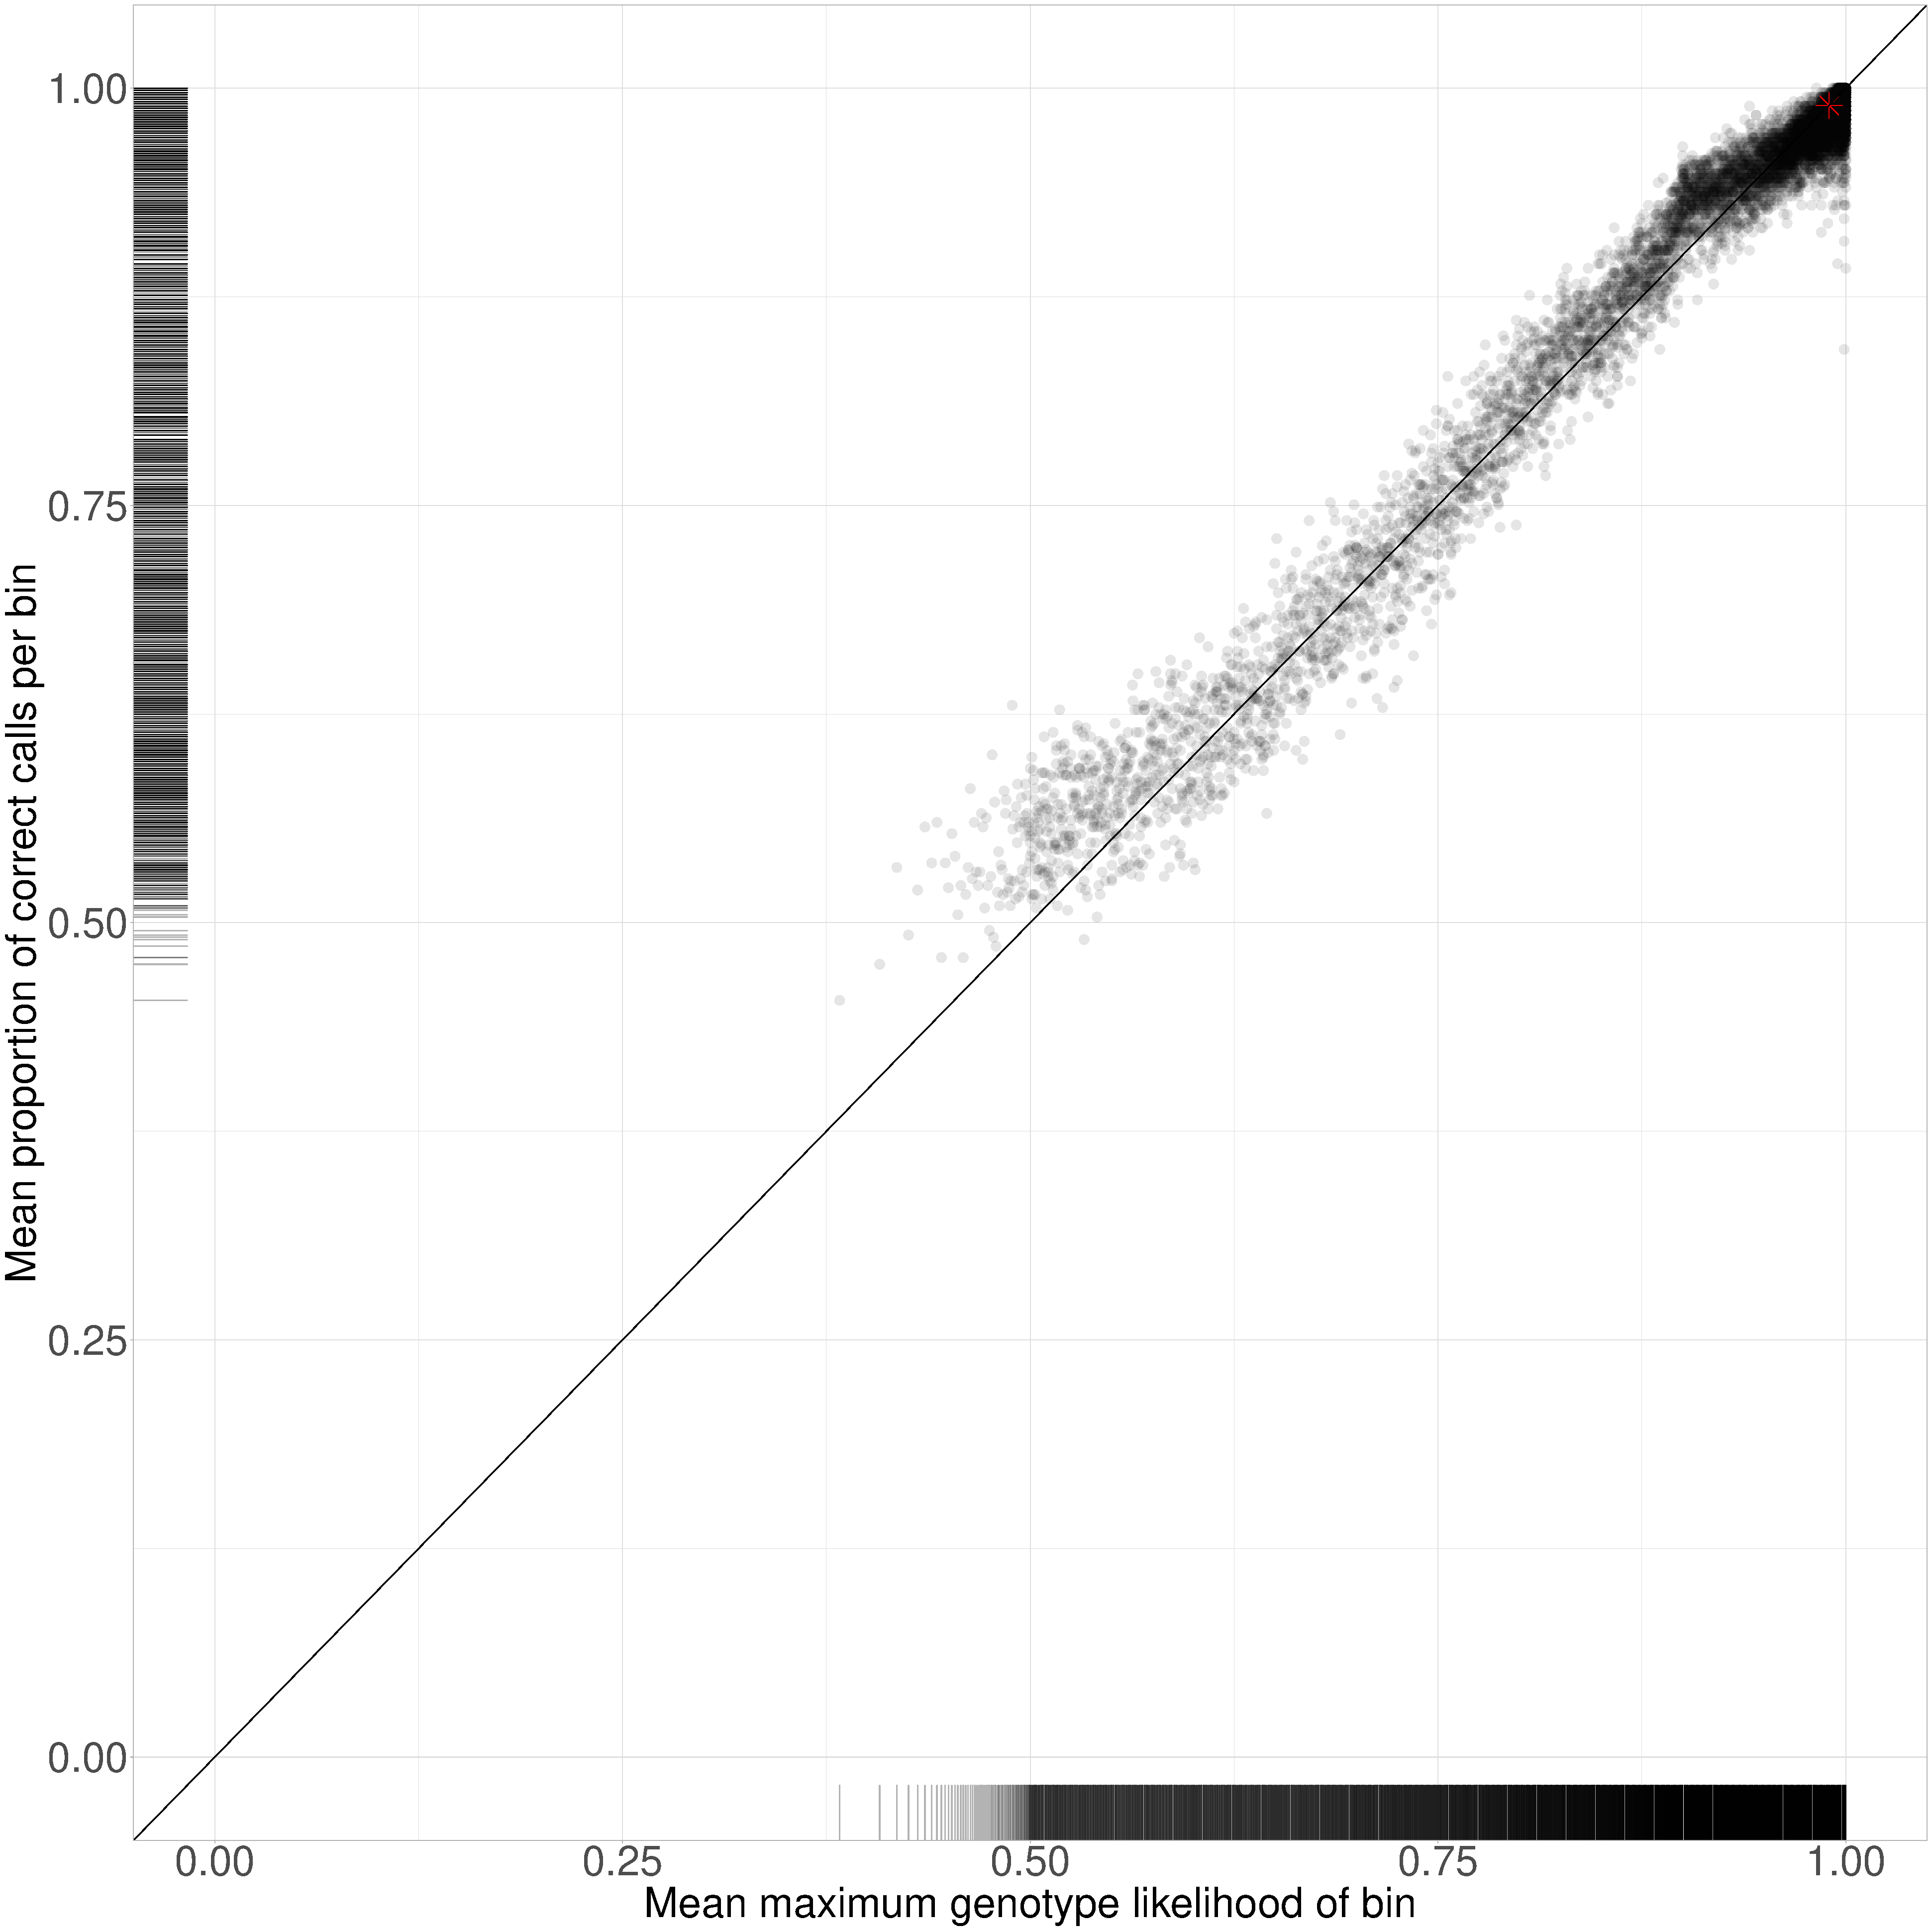
\includegraphics[width=1.0\textwidth]{../images/appendix/UstIshim_0.1x_bin.pdf}
    \caption{Relationship between genotype likelihood and probability of genotype call being correct for UstIshim downsampled to 0.1x coverage. Genome binned by maximum posterior genotype likelihood and mean maximum posterior genotype likelihood (x-axis) and proportion of correct calls per bin (y-axis). Rugs on each margin show the distribution of x and y values. Black line is $y=x$.}
    \label{fig:UstIshim_0.1x_bin}
\end{figure}

\begin{figure}[htp]
    \centering
    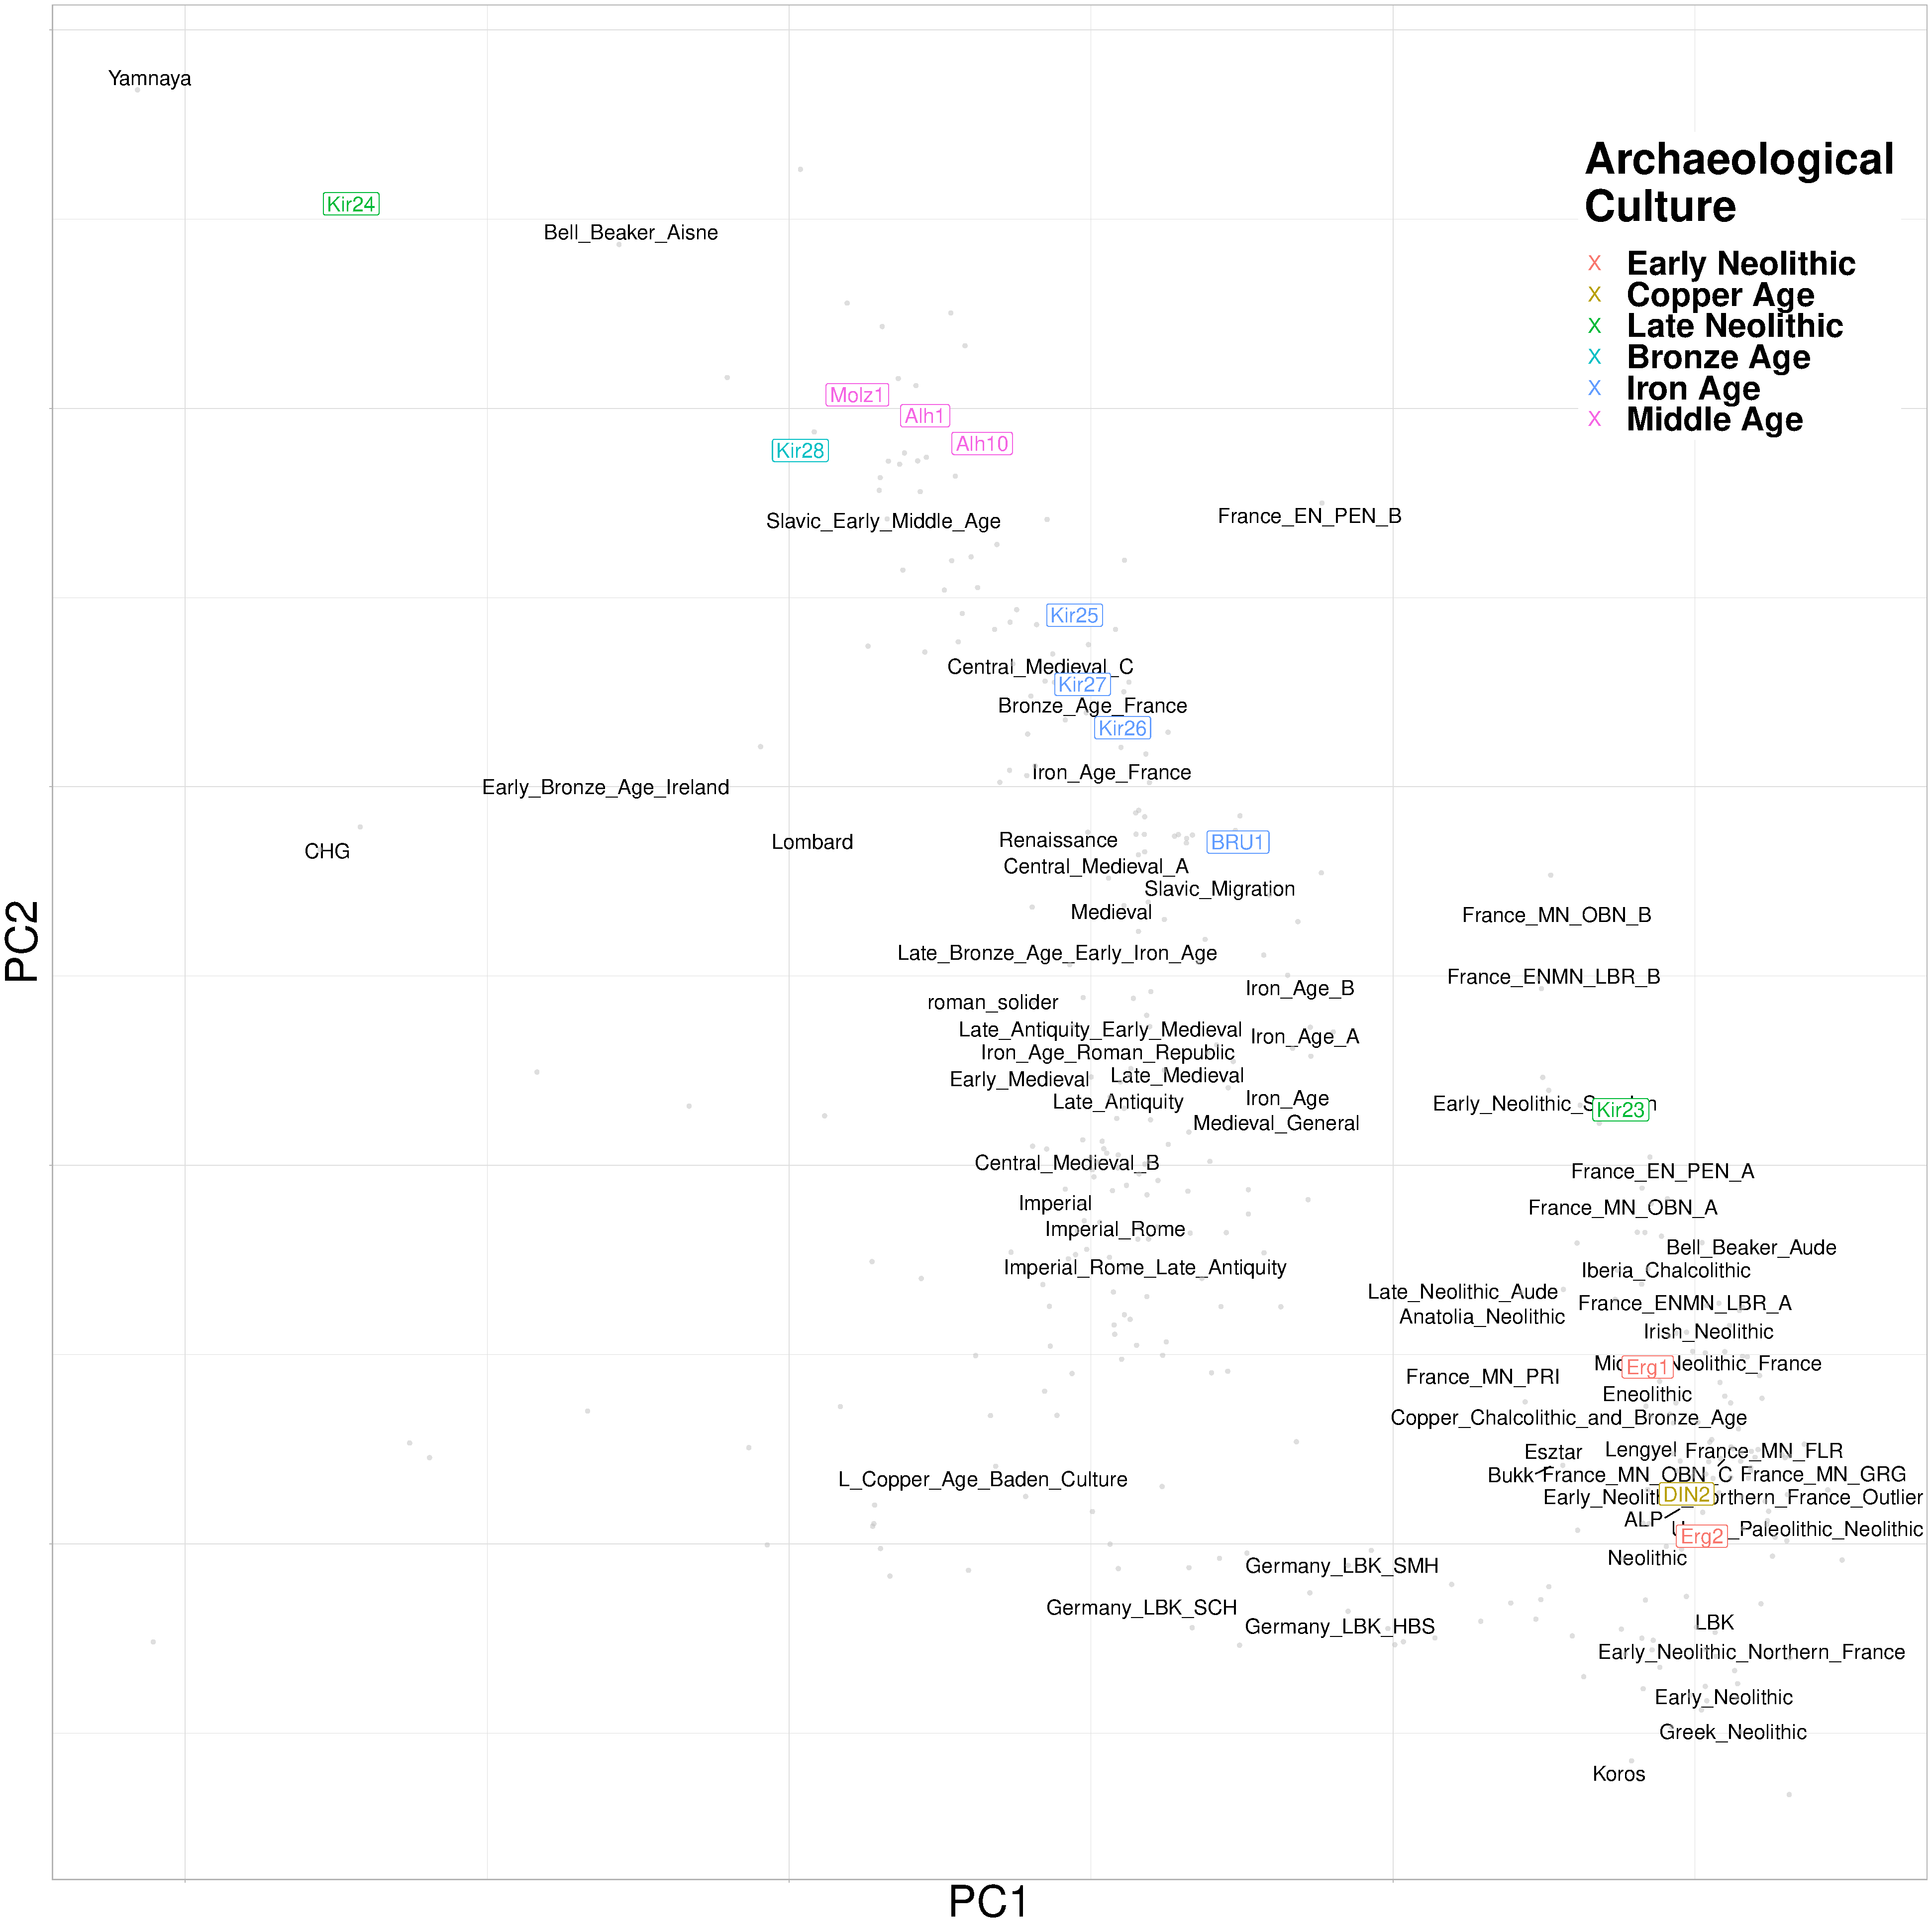
\includegraphics[width=1.0\textwidth]{../images/appendix/plink_withHG_PCA.pdf}
    \caption{Principle component analysis of genotype matrix using plink2. Grey points indicate principle component coordiantes for each sample. Black text indicated mean principle component coordinates for all individuals within that group. Coloured labels represent newly sequenced ancient samples. }
    \label{fig:plink_PCA_HG}
\end{figure}

\begin{figure}[htp]
    \centering
    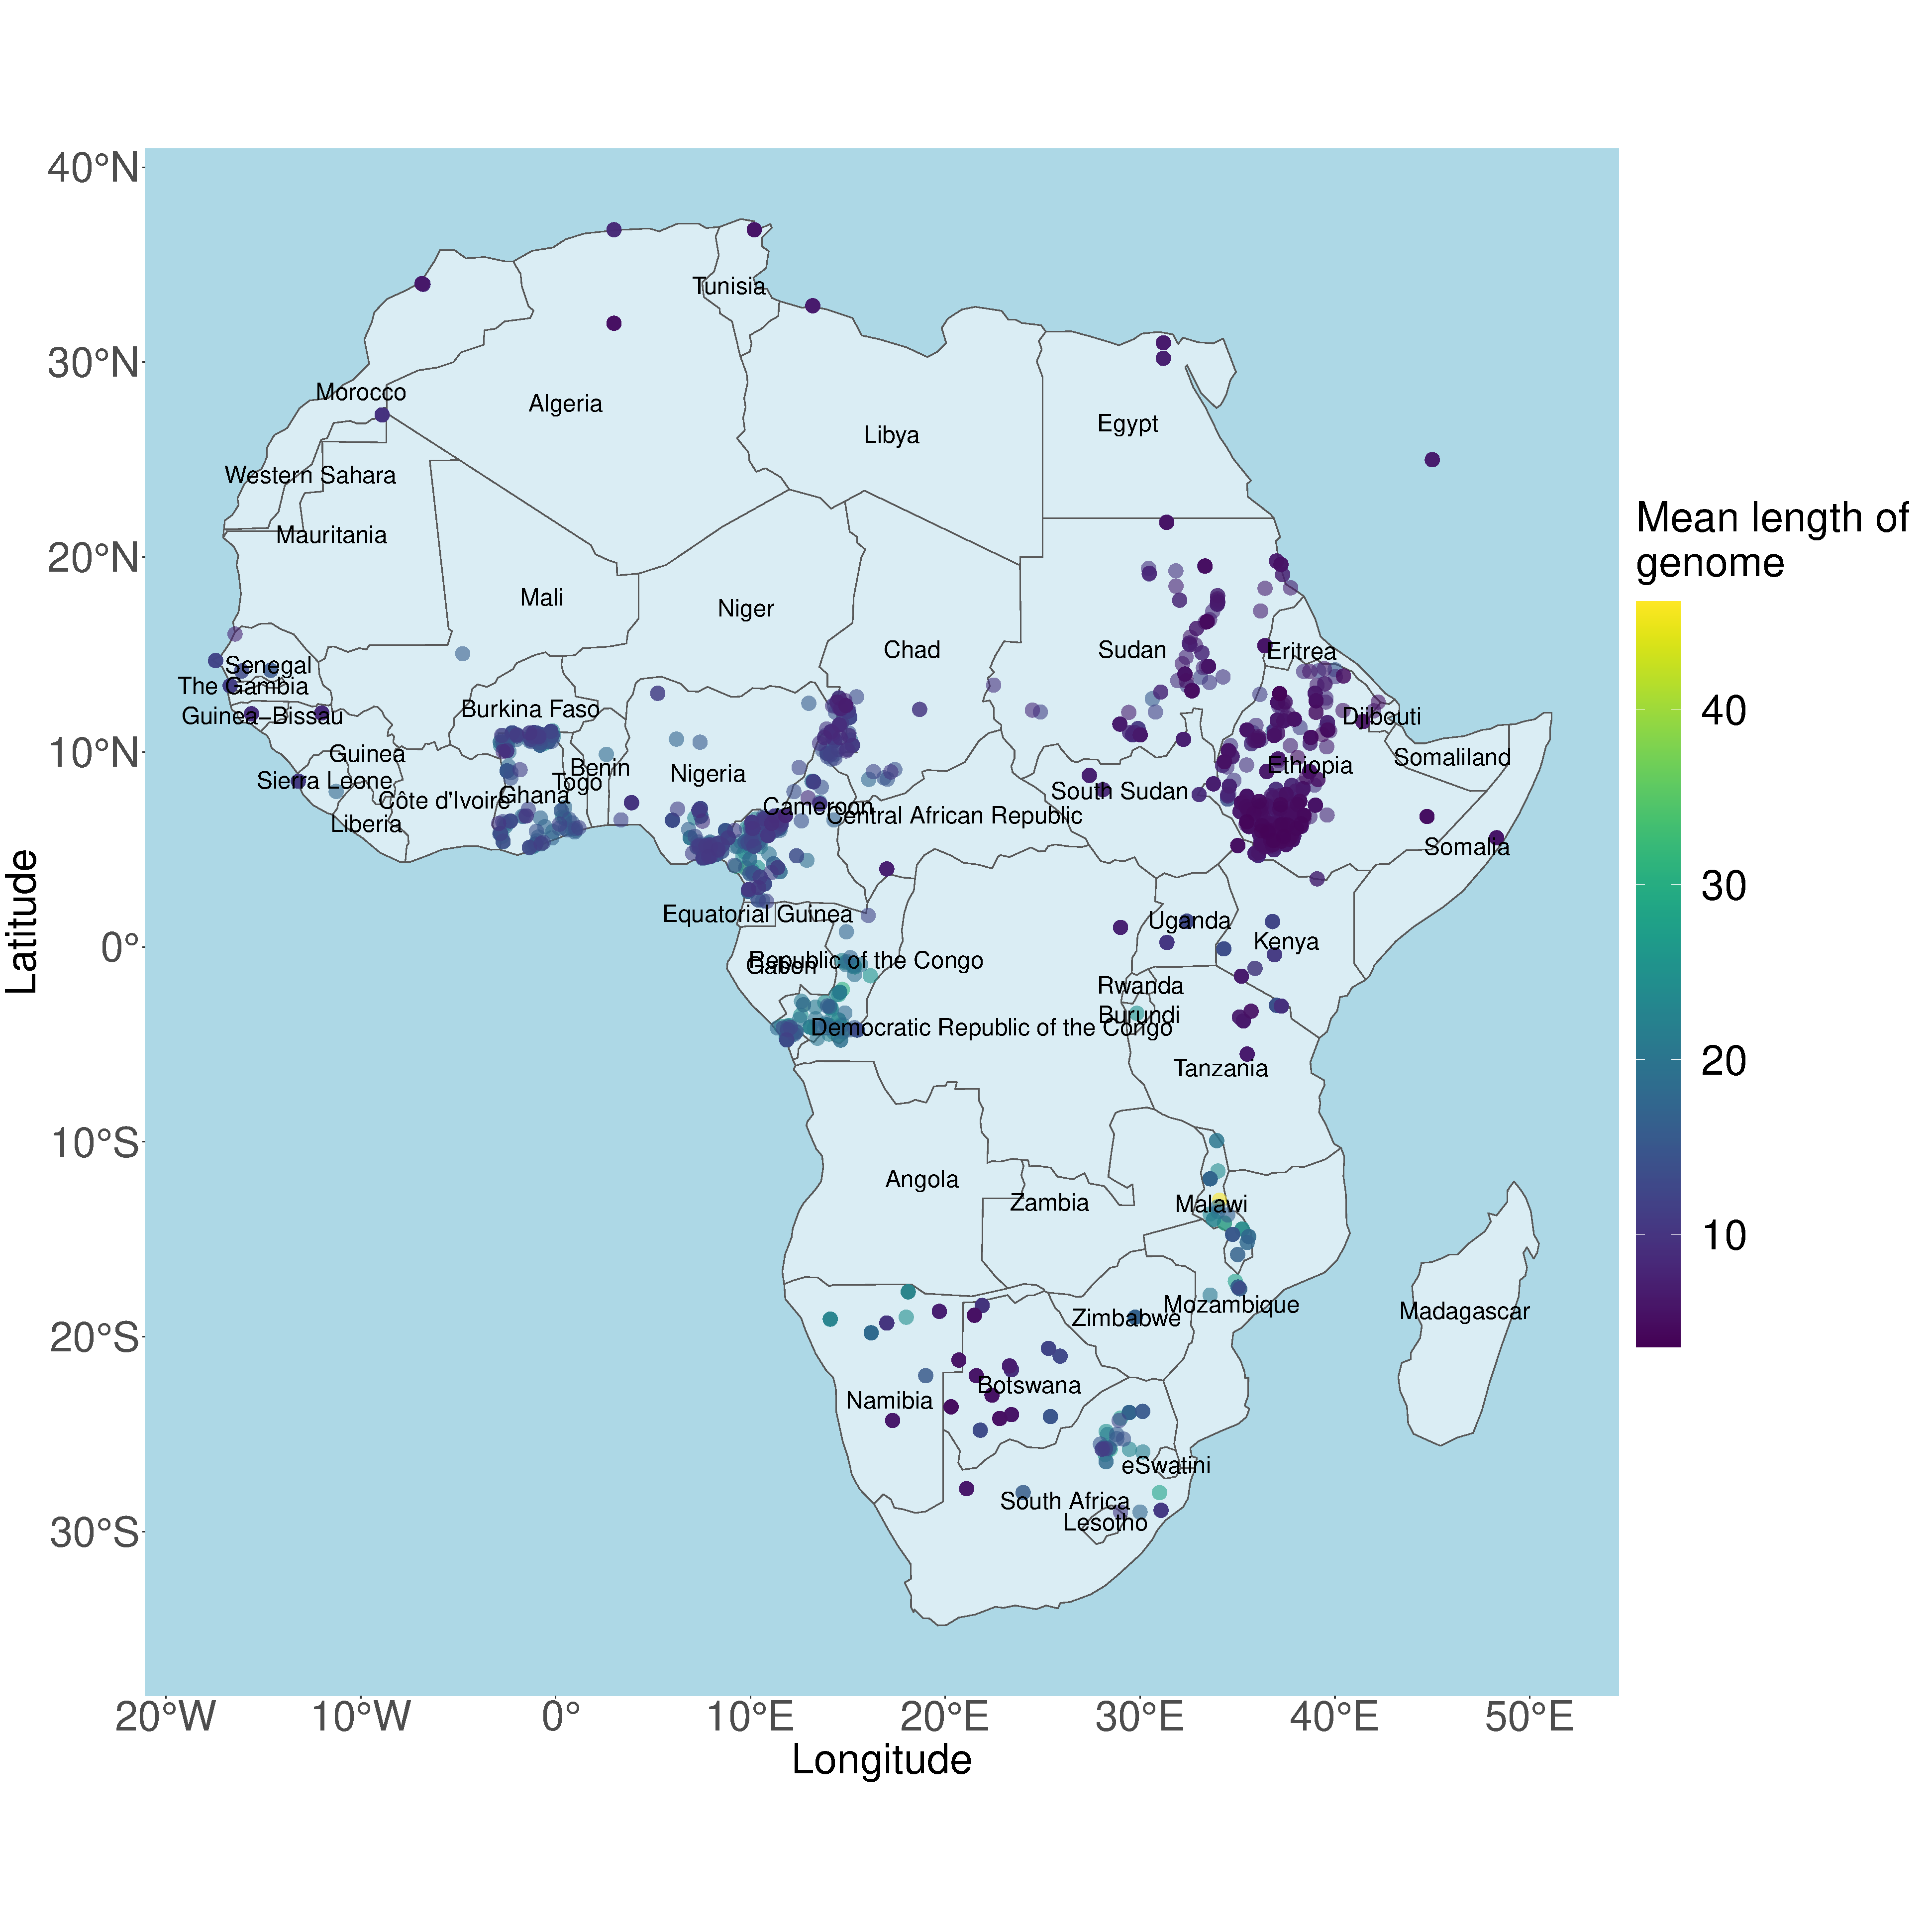
\includegraphics[width=1.0\textwidth]{../images/appendix/haplotype_map_Brazil.pdf}
    \caption{Map of haplotype donation to U.K. Biobank individuals born in Brazil. Each point represents one Human Origins population, coloured according to the summed amount of chunklengths that population donates to all U.K. Biobank individuals born in Brazil.}
    \label{fig:haplotype_map_Brazil}
\end{figure}

\begin{figure}[htp]
    \centering
    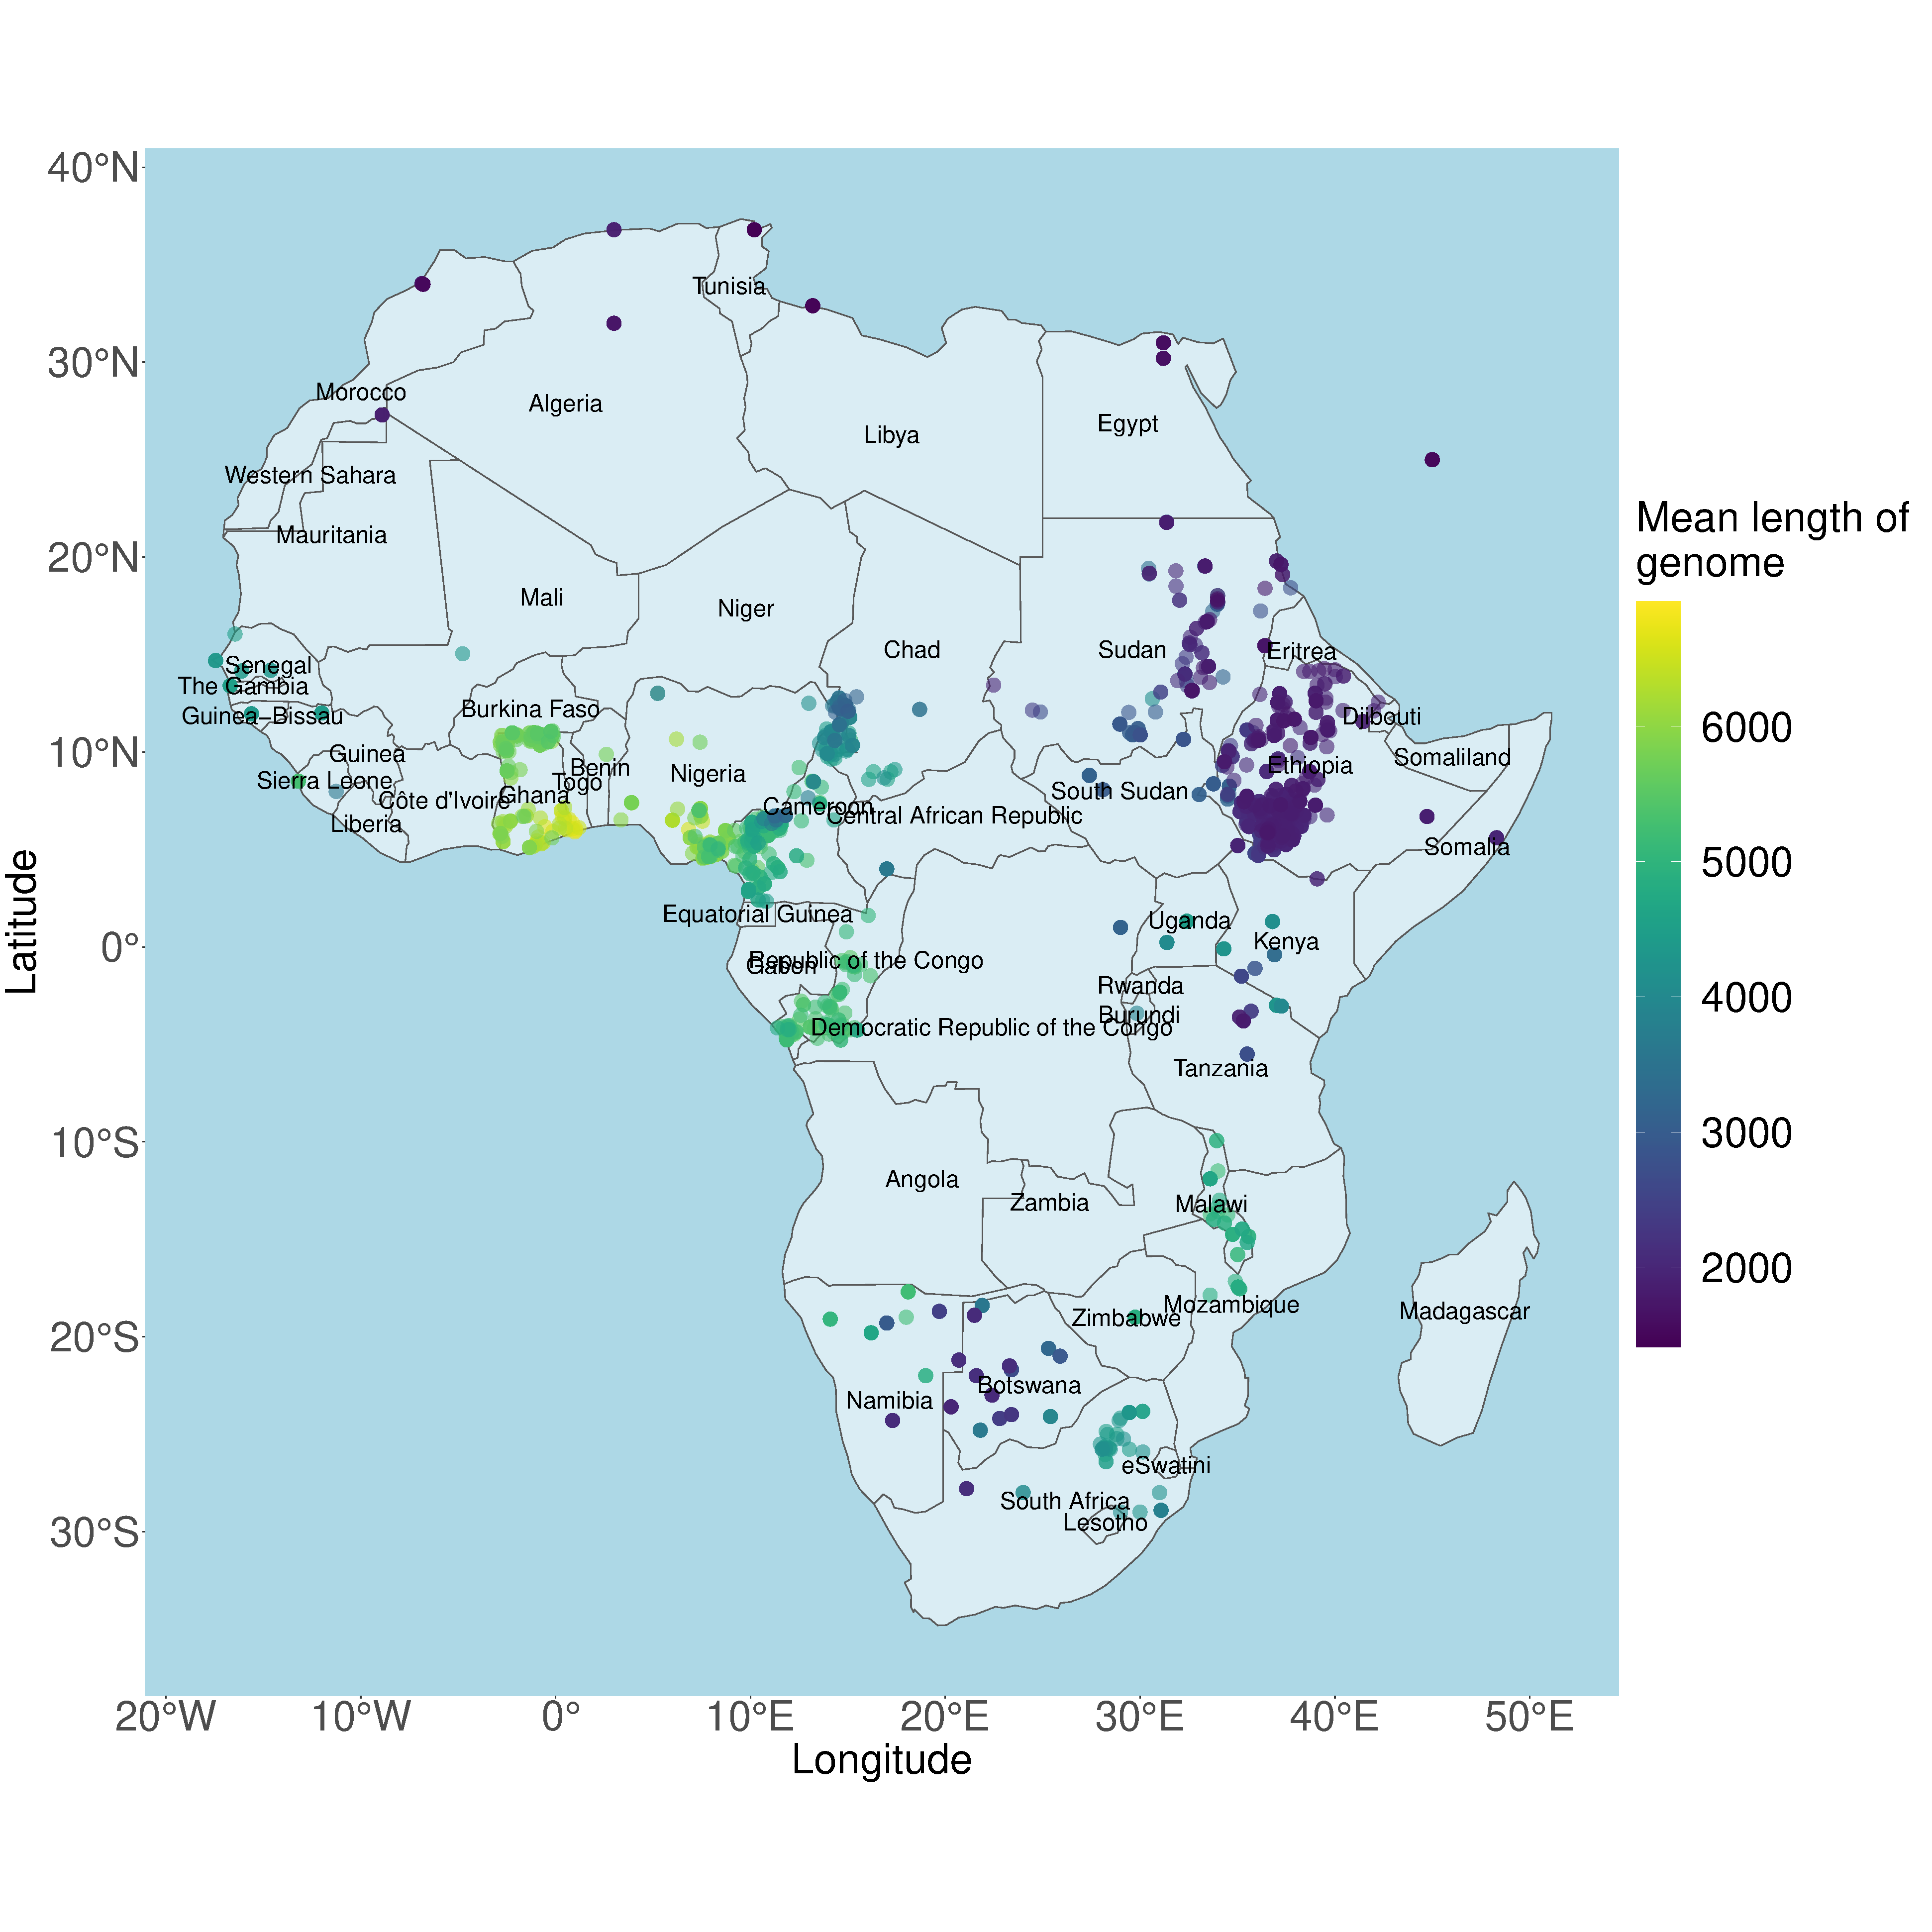
\includegraphics[width=1.0\textwidth]{../images/appendix/haplotype_map_Caribbean.pdf}
    \caption{Map of haplotype donation to U.K. Biobank individuals born in the Caribbean. Each point represents one Human Origins population, coloured according to the summed amount of chunklengths that population donates to all U.K. Biobank individuals born in the Caribbean.}
    \label{fig:haplotype_map_Caribbean}
\end{figure}

\begin{figure}[htp]
    \centering
    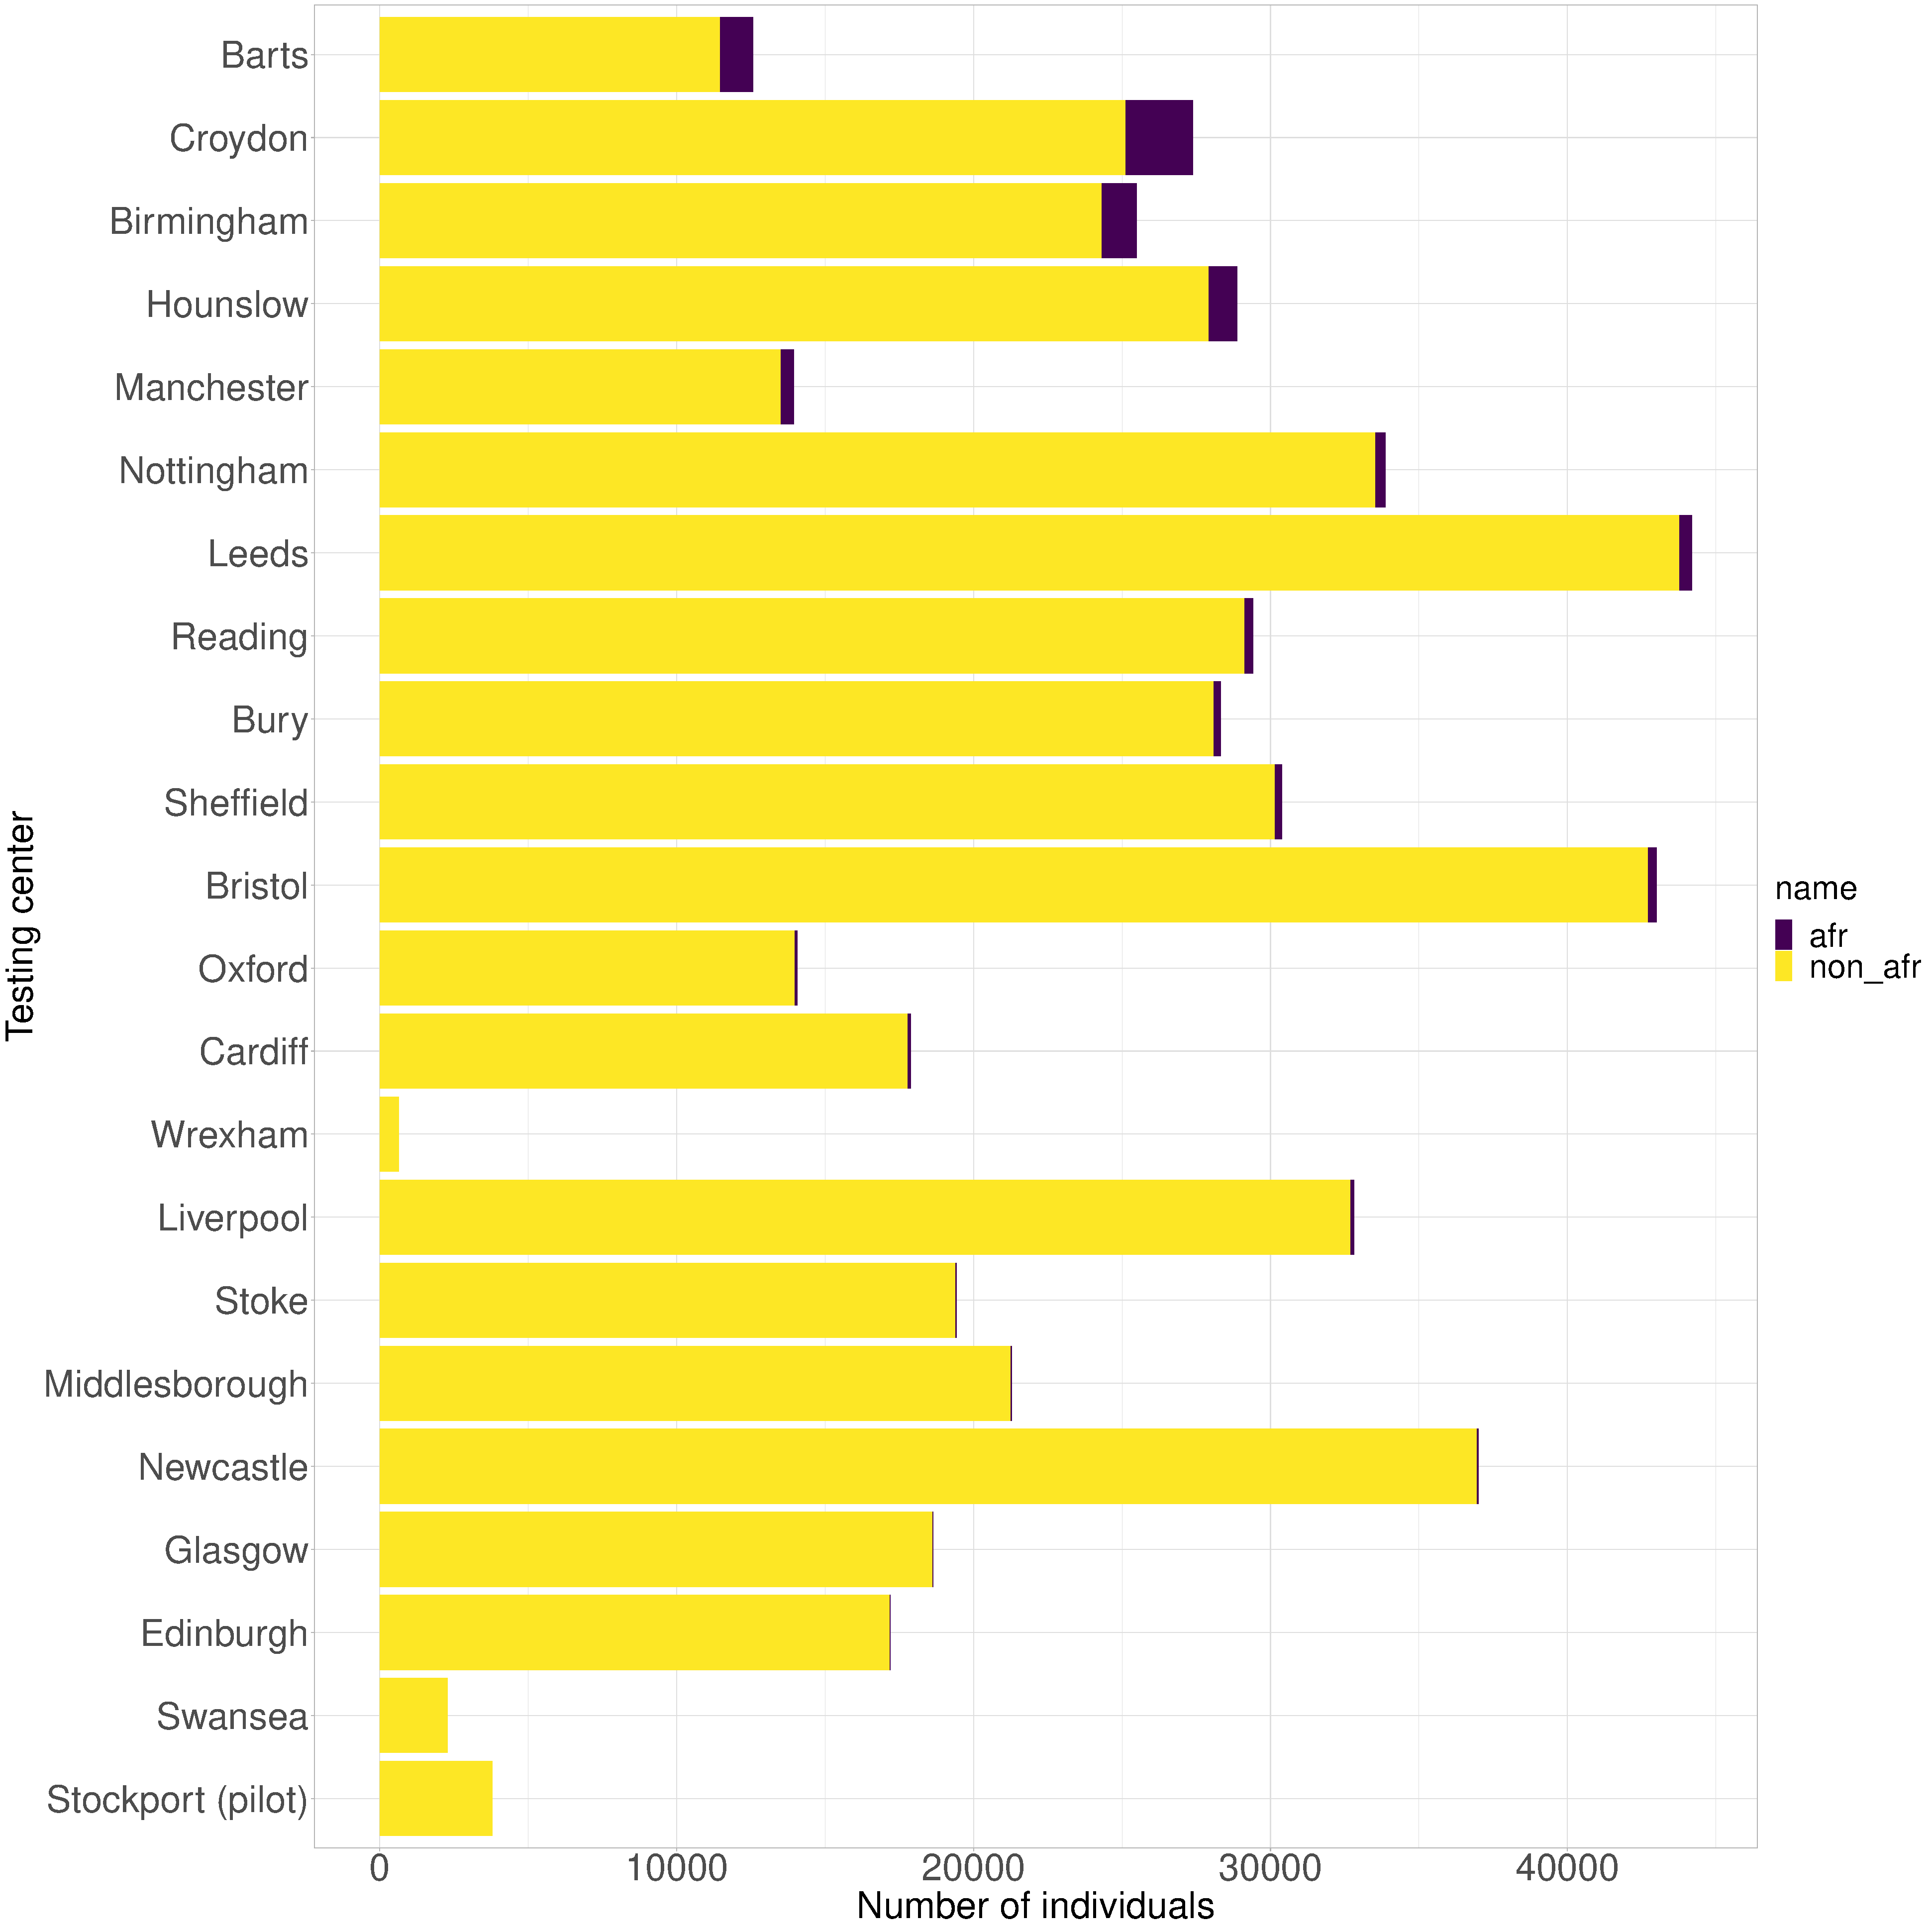
\includegraphics[width=1.0\textwidth]{../images/appendix/testing_centre_afr_prop.pdf}
    \caption{Number of individuals who have (purple) and have not (yellow) at least 50\% African ancestry (purple) by different testing centers. Centers ordered by proportion of individuals who have at least 50\% African ancestry.}
    \label{fig:testing_centre_afr_prop}
\end{figure}

\begin{figure}[htp]
    \centering
    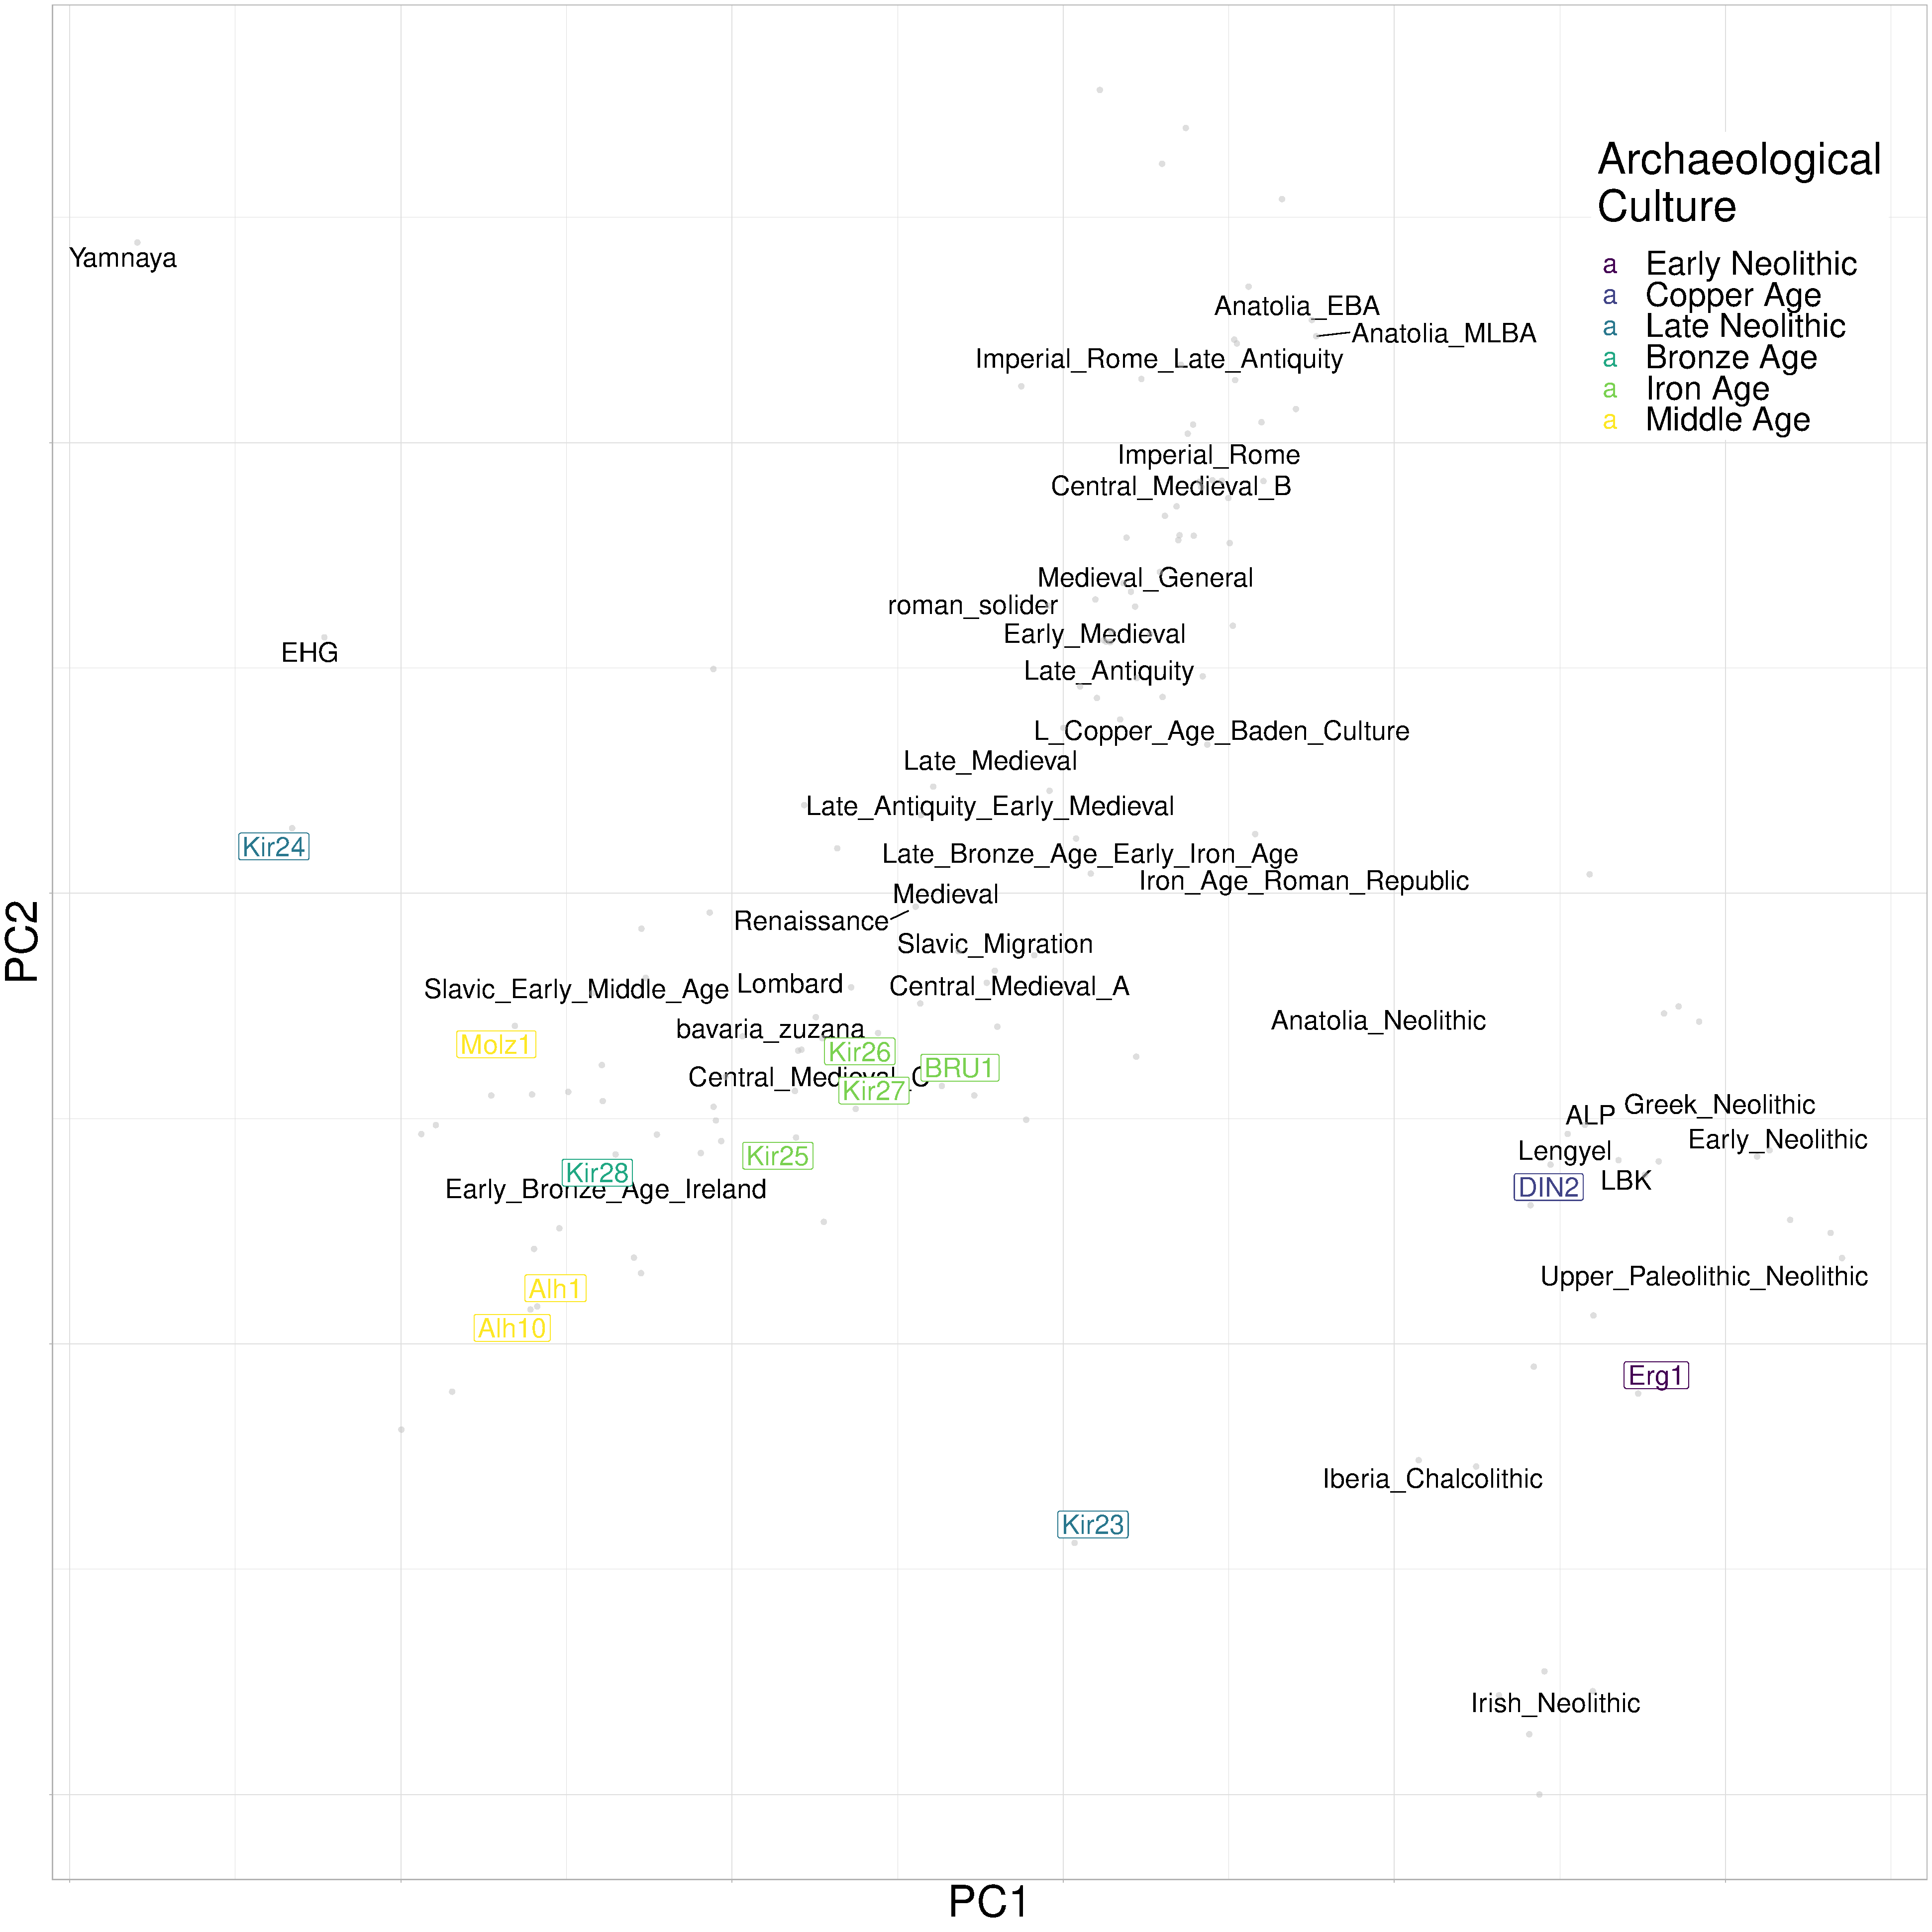
\includegraphics[width=1.0\textwidth]{../images/appendix/chromopainter_PCA_ancients_Bavaria.pdf}
    \caption{Principle Component Analysis on chunklengths matrix of newly sequenced ancient Bavarian samples and selected ancient literature samples.}
    \label{fig:chromopainter_PCA_ancients_Bavaria}
\end{figure}

\begin{figure}[htp]
    \centering
    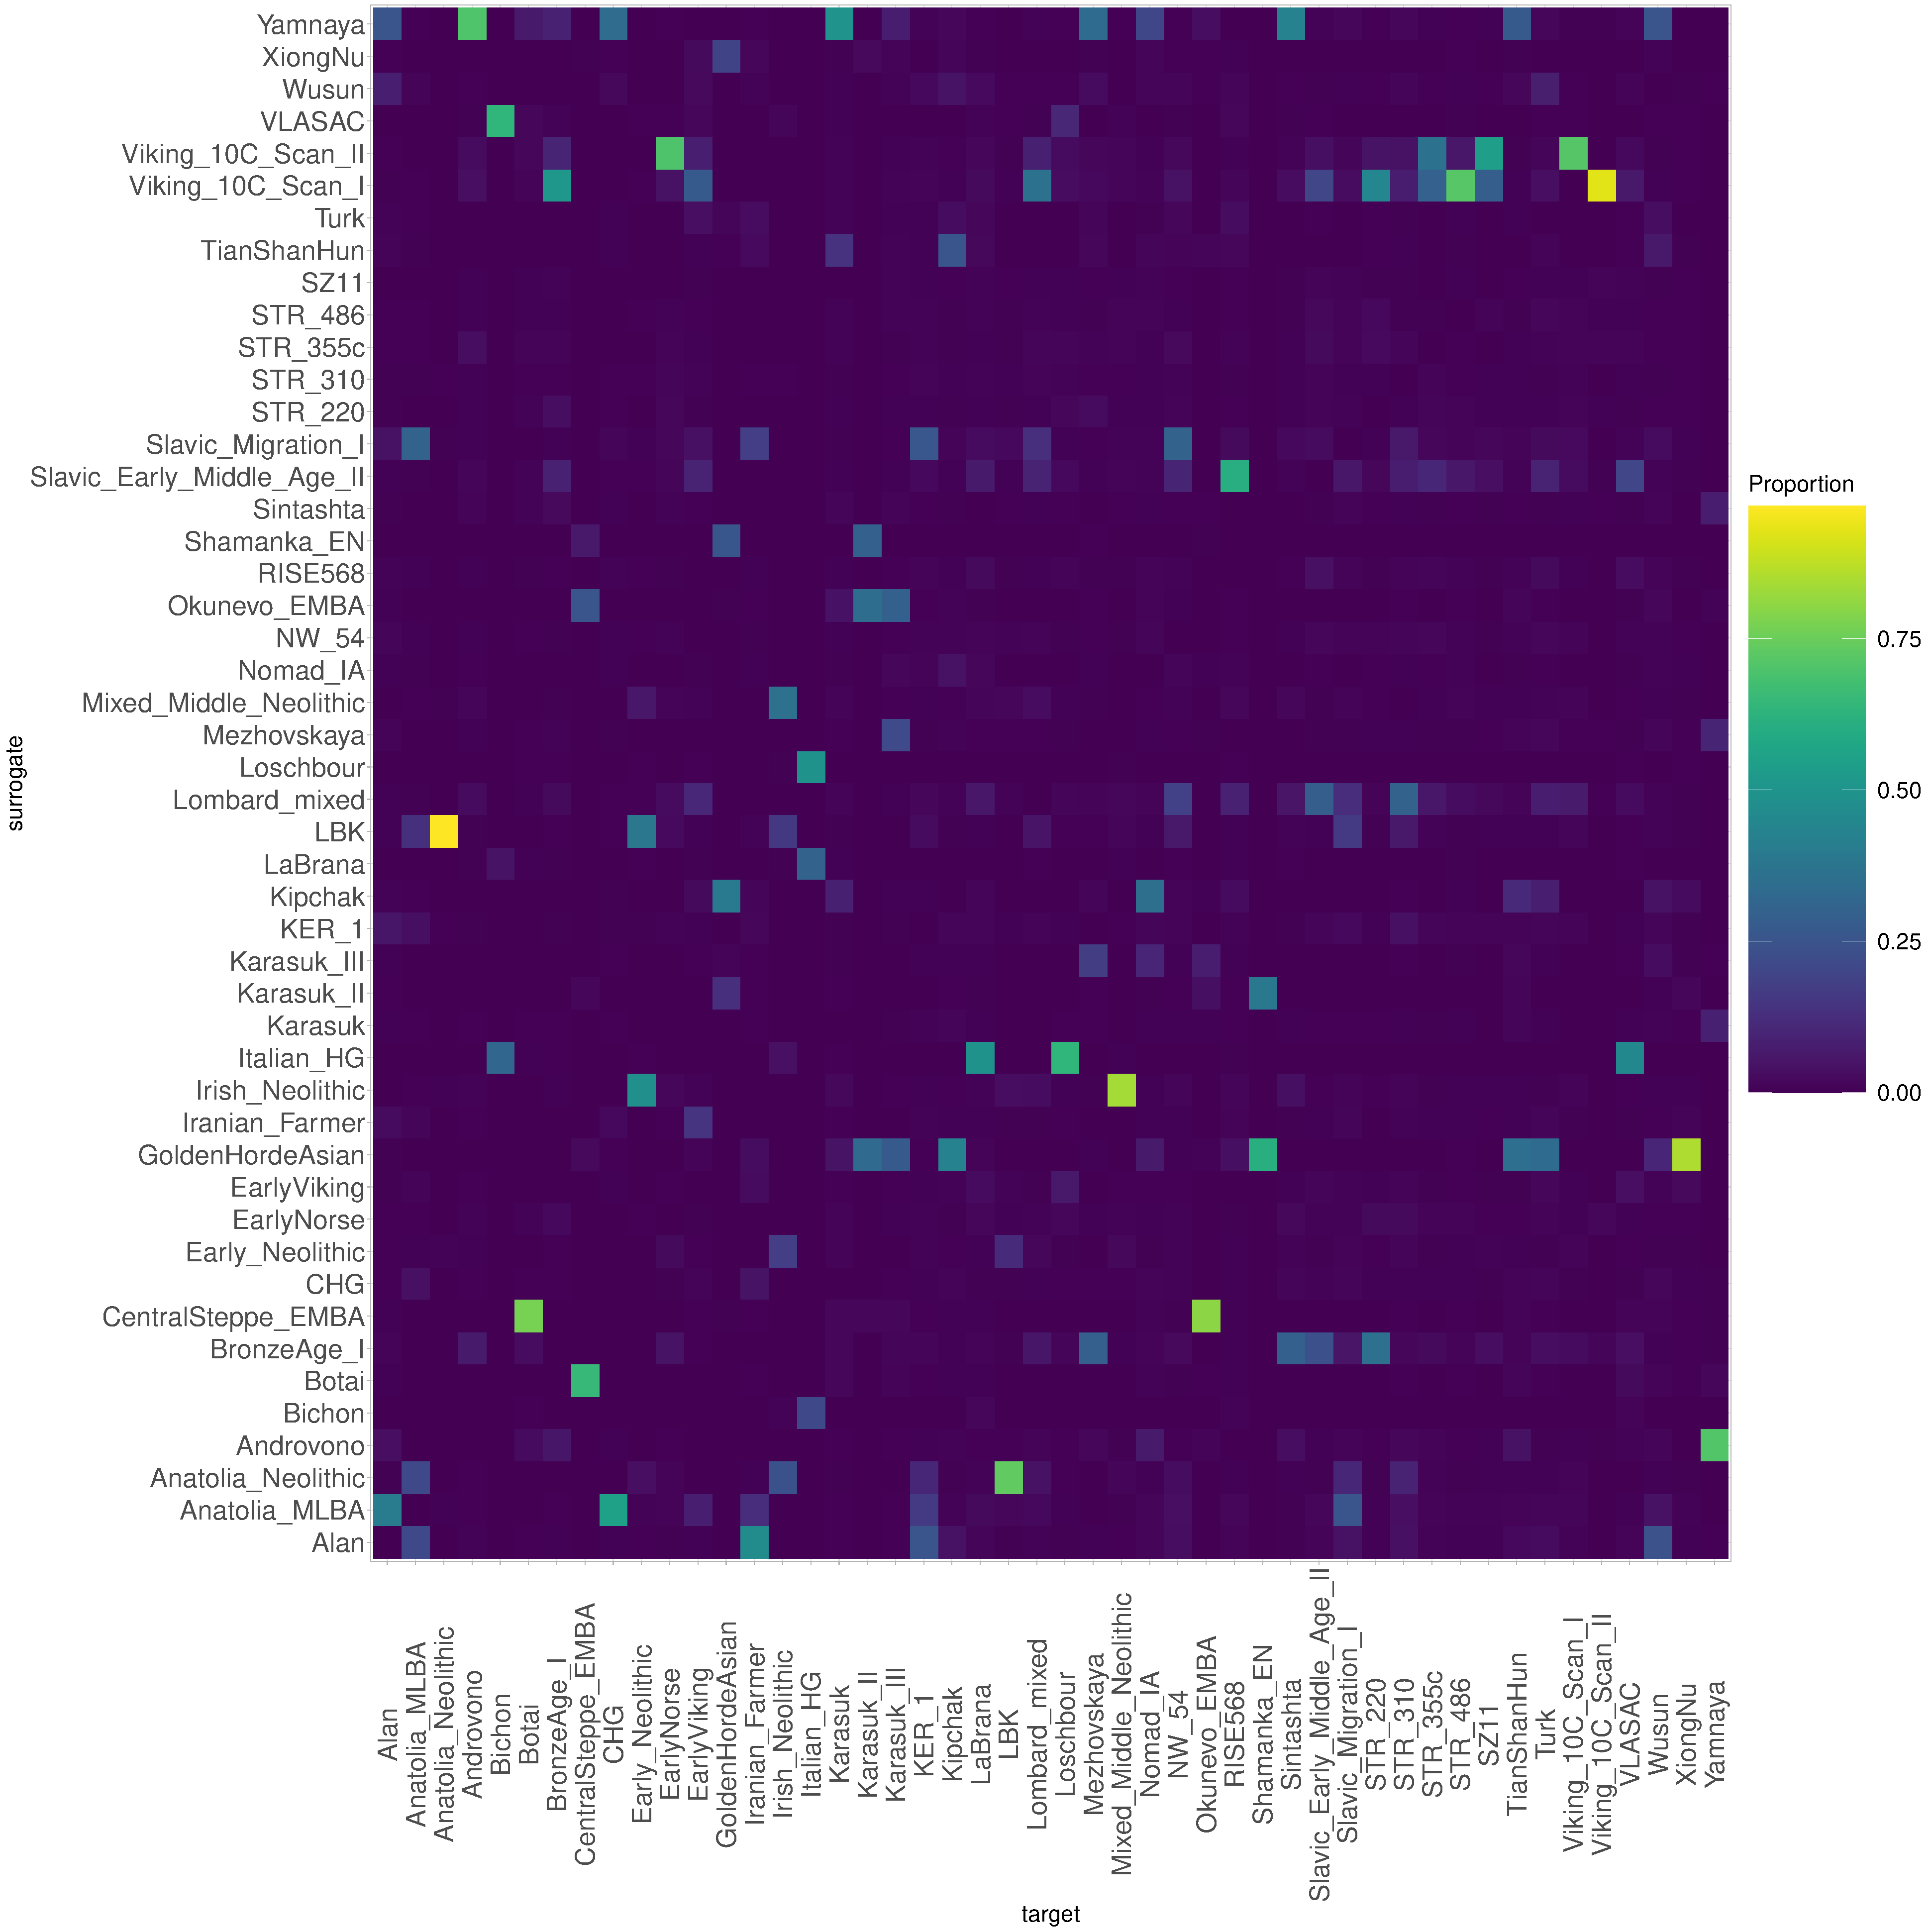
\includegraphics[width=1.0\textwidth]{../images/appendix/SF_heatmap_slavs.pdf}
    \caption{Heatmap of SOURCEFIND proportions for all clusters in the ancient Slav analysis.}
    \label{fig:SF_heatmap_slavs}
\end{figure}


\chapter{Supplementary results} \label{appendixlabel5}

Auxiliary results.

\subsection{Determining the number of MCMC iterations required in SOURCEFIND analysis} \label{sec:SF_test_iterations}

SOURCEFIND is a haplotype-based method for inferring ancestry. At its heart, SOURCEFIND uses Markov chain Monte Carlo sampling to explore the parameter space of ancestry proportions. As is the case with any method that uses MCMC sampling, it is important to ensure that enough iterations have been performed; if this is not the case, the algorithm may not converge.

To determine what is the minimum number of iterations, I ran SOURCEFIND for 7 different numbers of iterations and 10 runs for each number. Results are presented in Figure \ref{fig:iterations}. Visually inspecting the results shows that using 50,000 iterations or less leads to variable results. 500,000 iterations appears to be the best balance between running time and accuracy. 

\begin{figure}[htp]
    \centering
    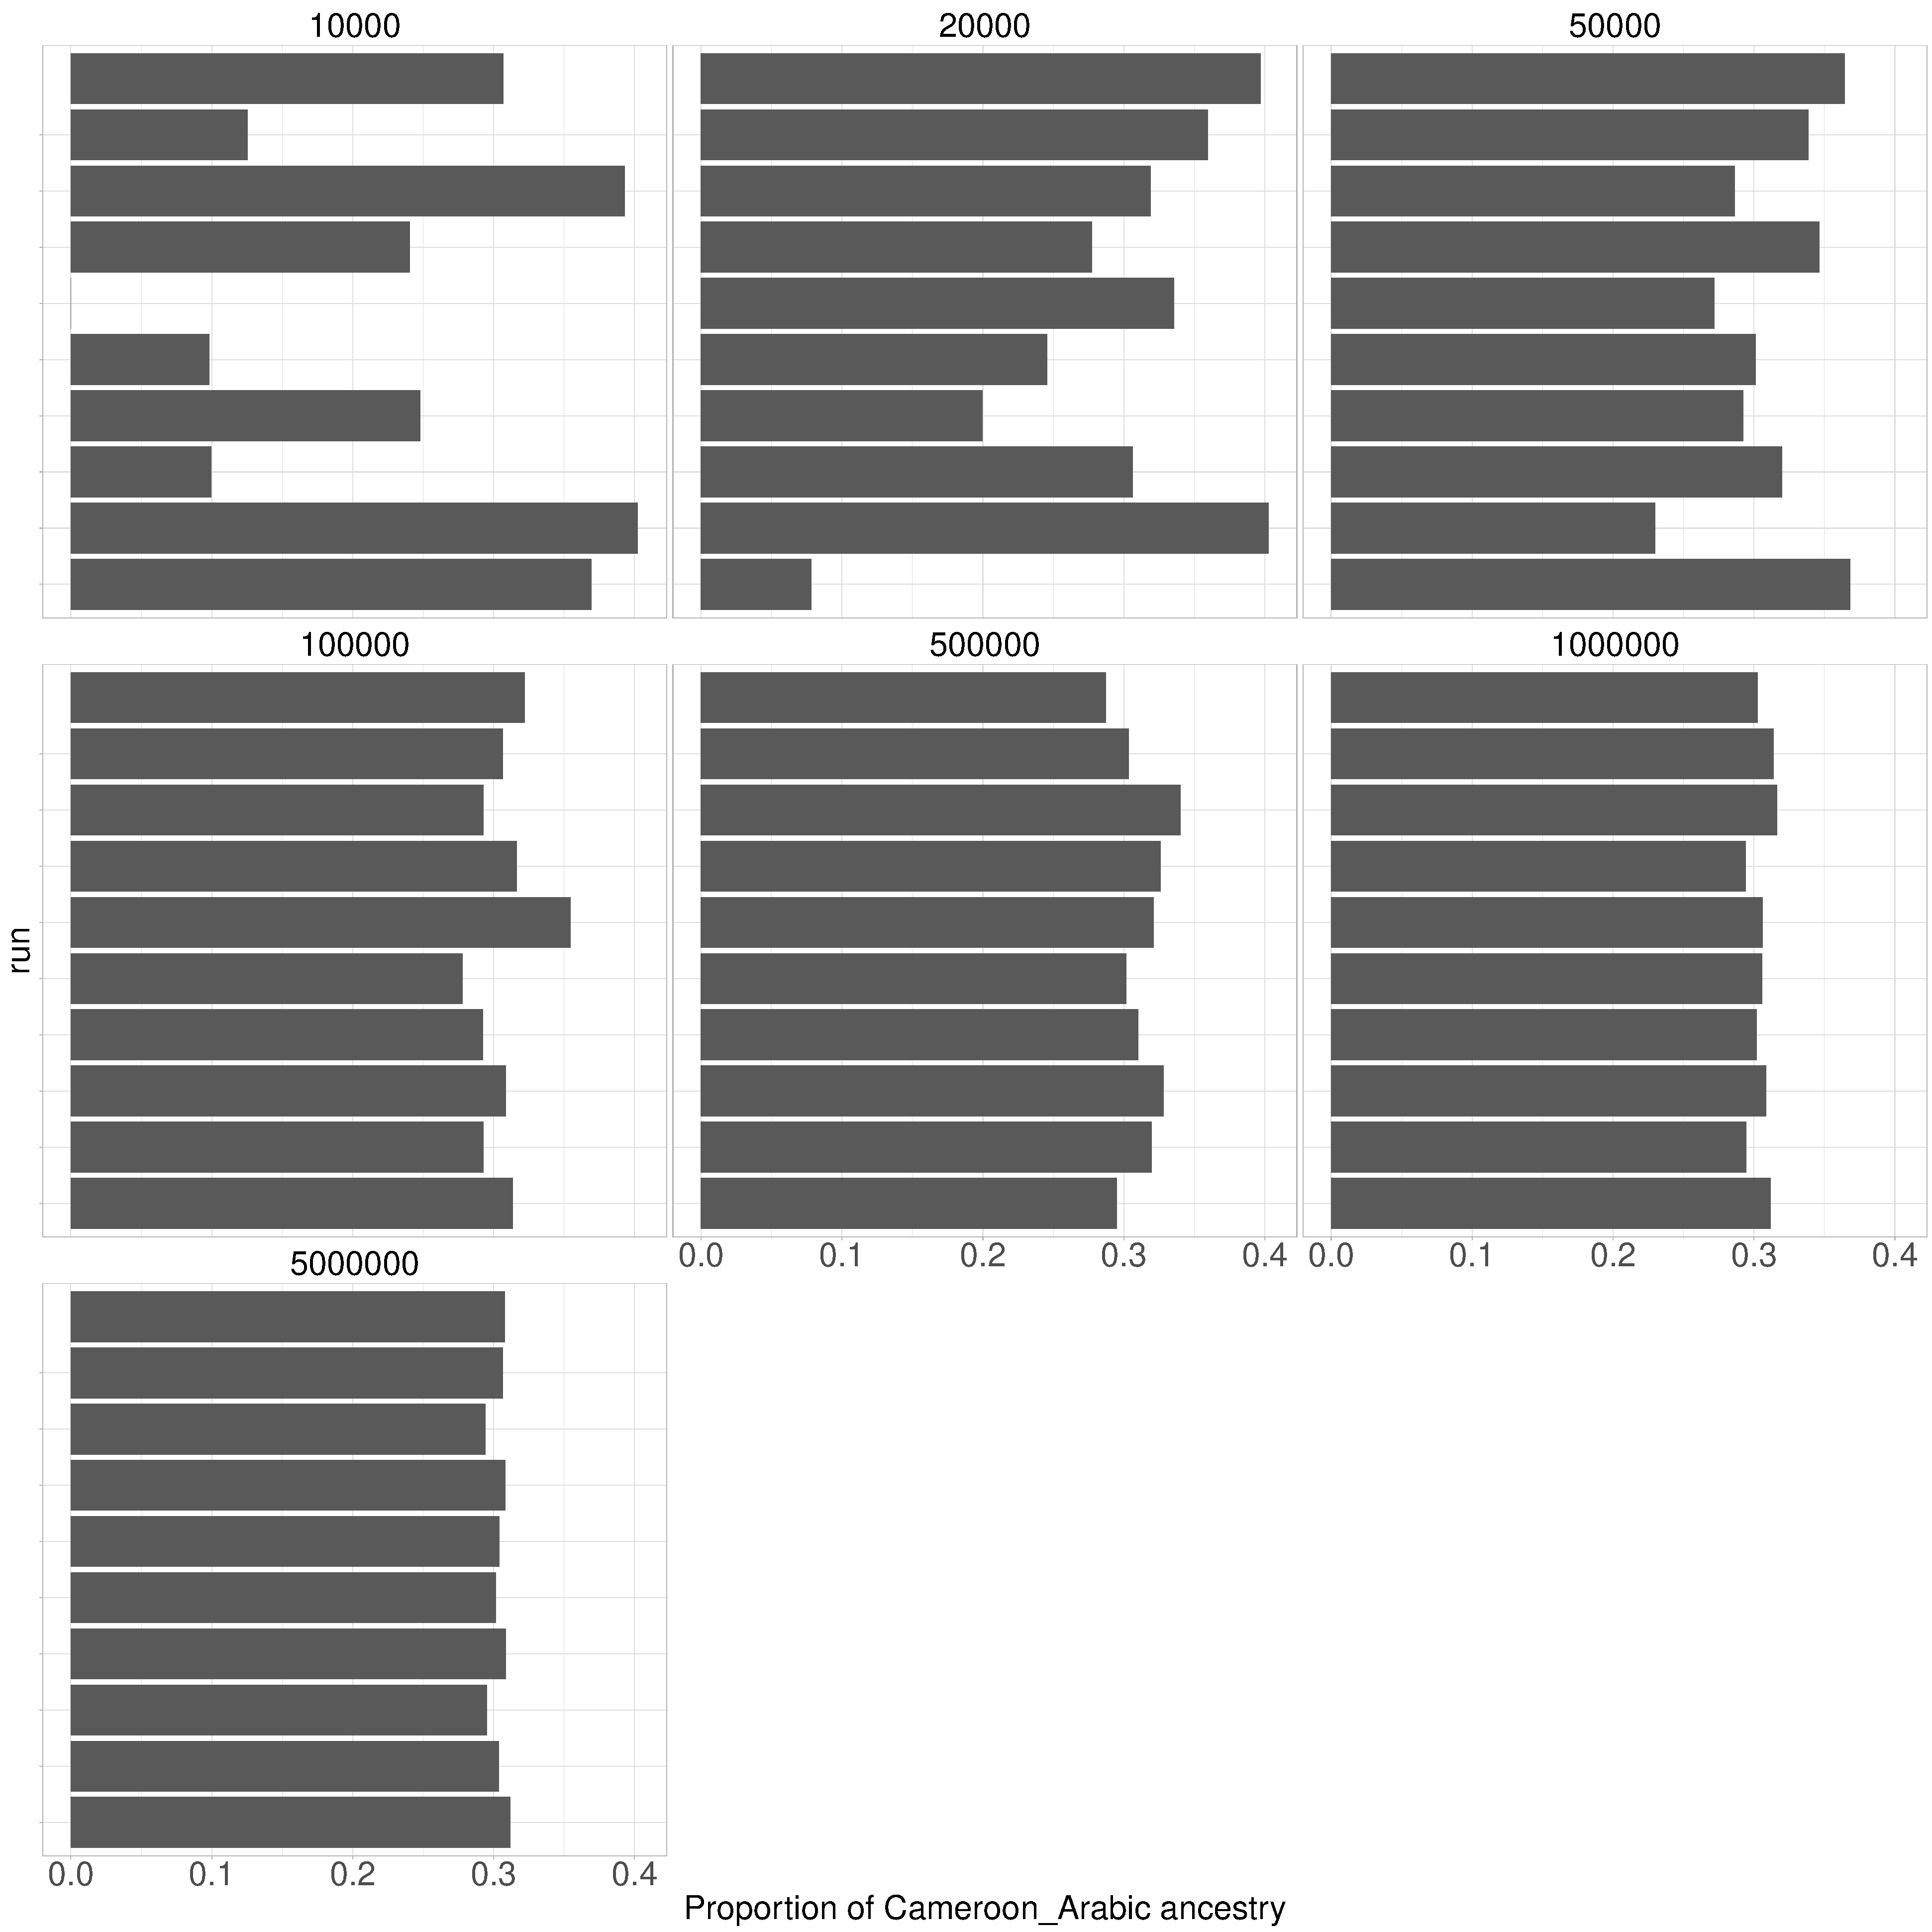
\includegraphics[width=1.0\textwidth]{../images/appendix/iterations.pdf}
    \caption{Proportion of inferred Cameroon Arabic ancestry averaged across individuals from Cameroon Kanuri ethnic group. Each panel contains proportions for a different number of MCMC iterations. Within each panel, each bar is the proportion inferred from each of the 10 independent SOURCEFIND runs.}
    \label{fig:iterations}
\end{figure}

\subsection{Determining the number of SNPs required to separate individuals from Devon and Cornwall} 
\label{sec:SNP_Count_Assignment_DevCorn}

This figure shows the how TVD assignment accuracy varies with the total number of SNPs included.


\begin{figure}[htp]
    \centering
    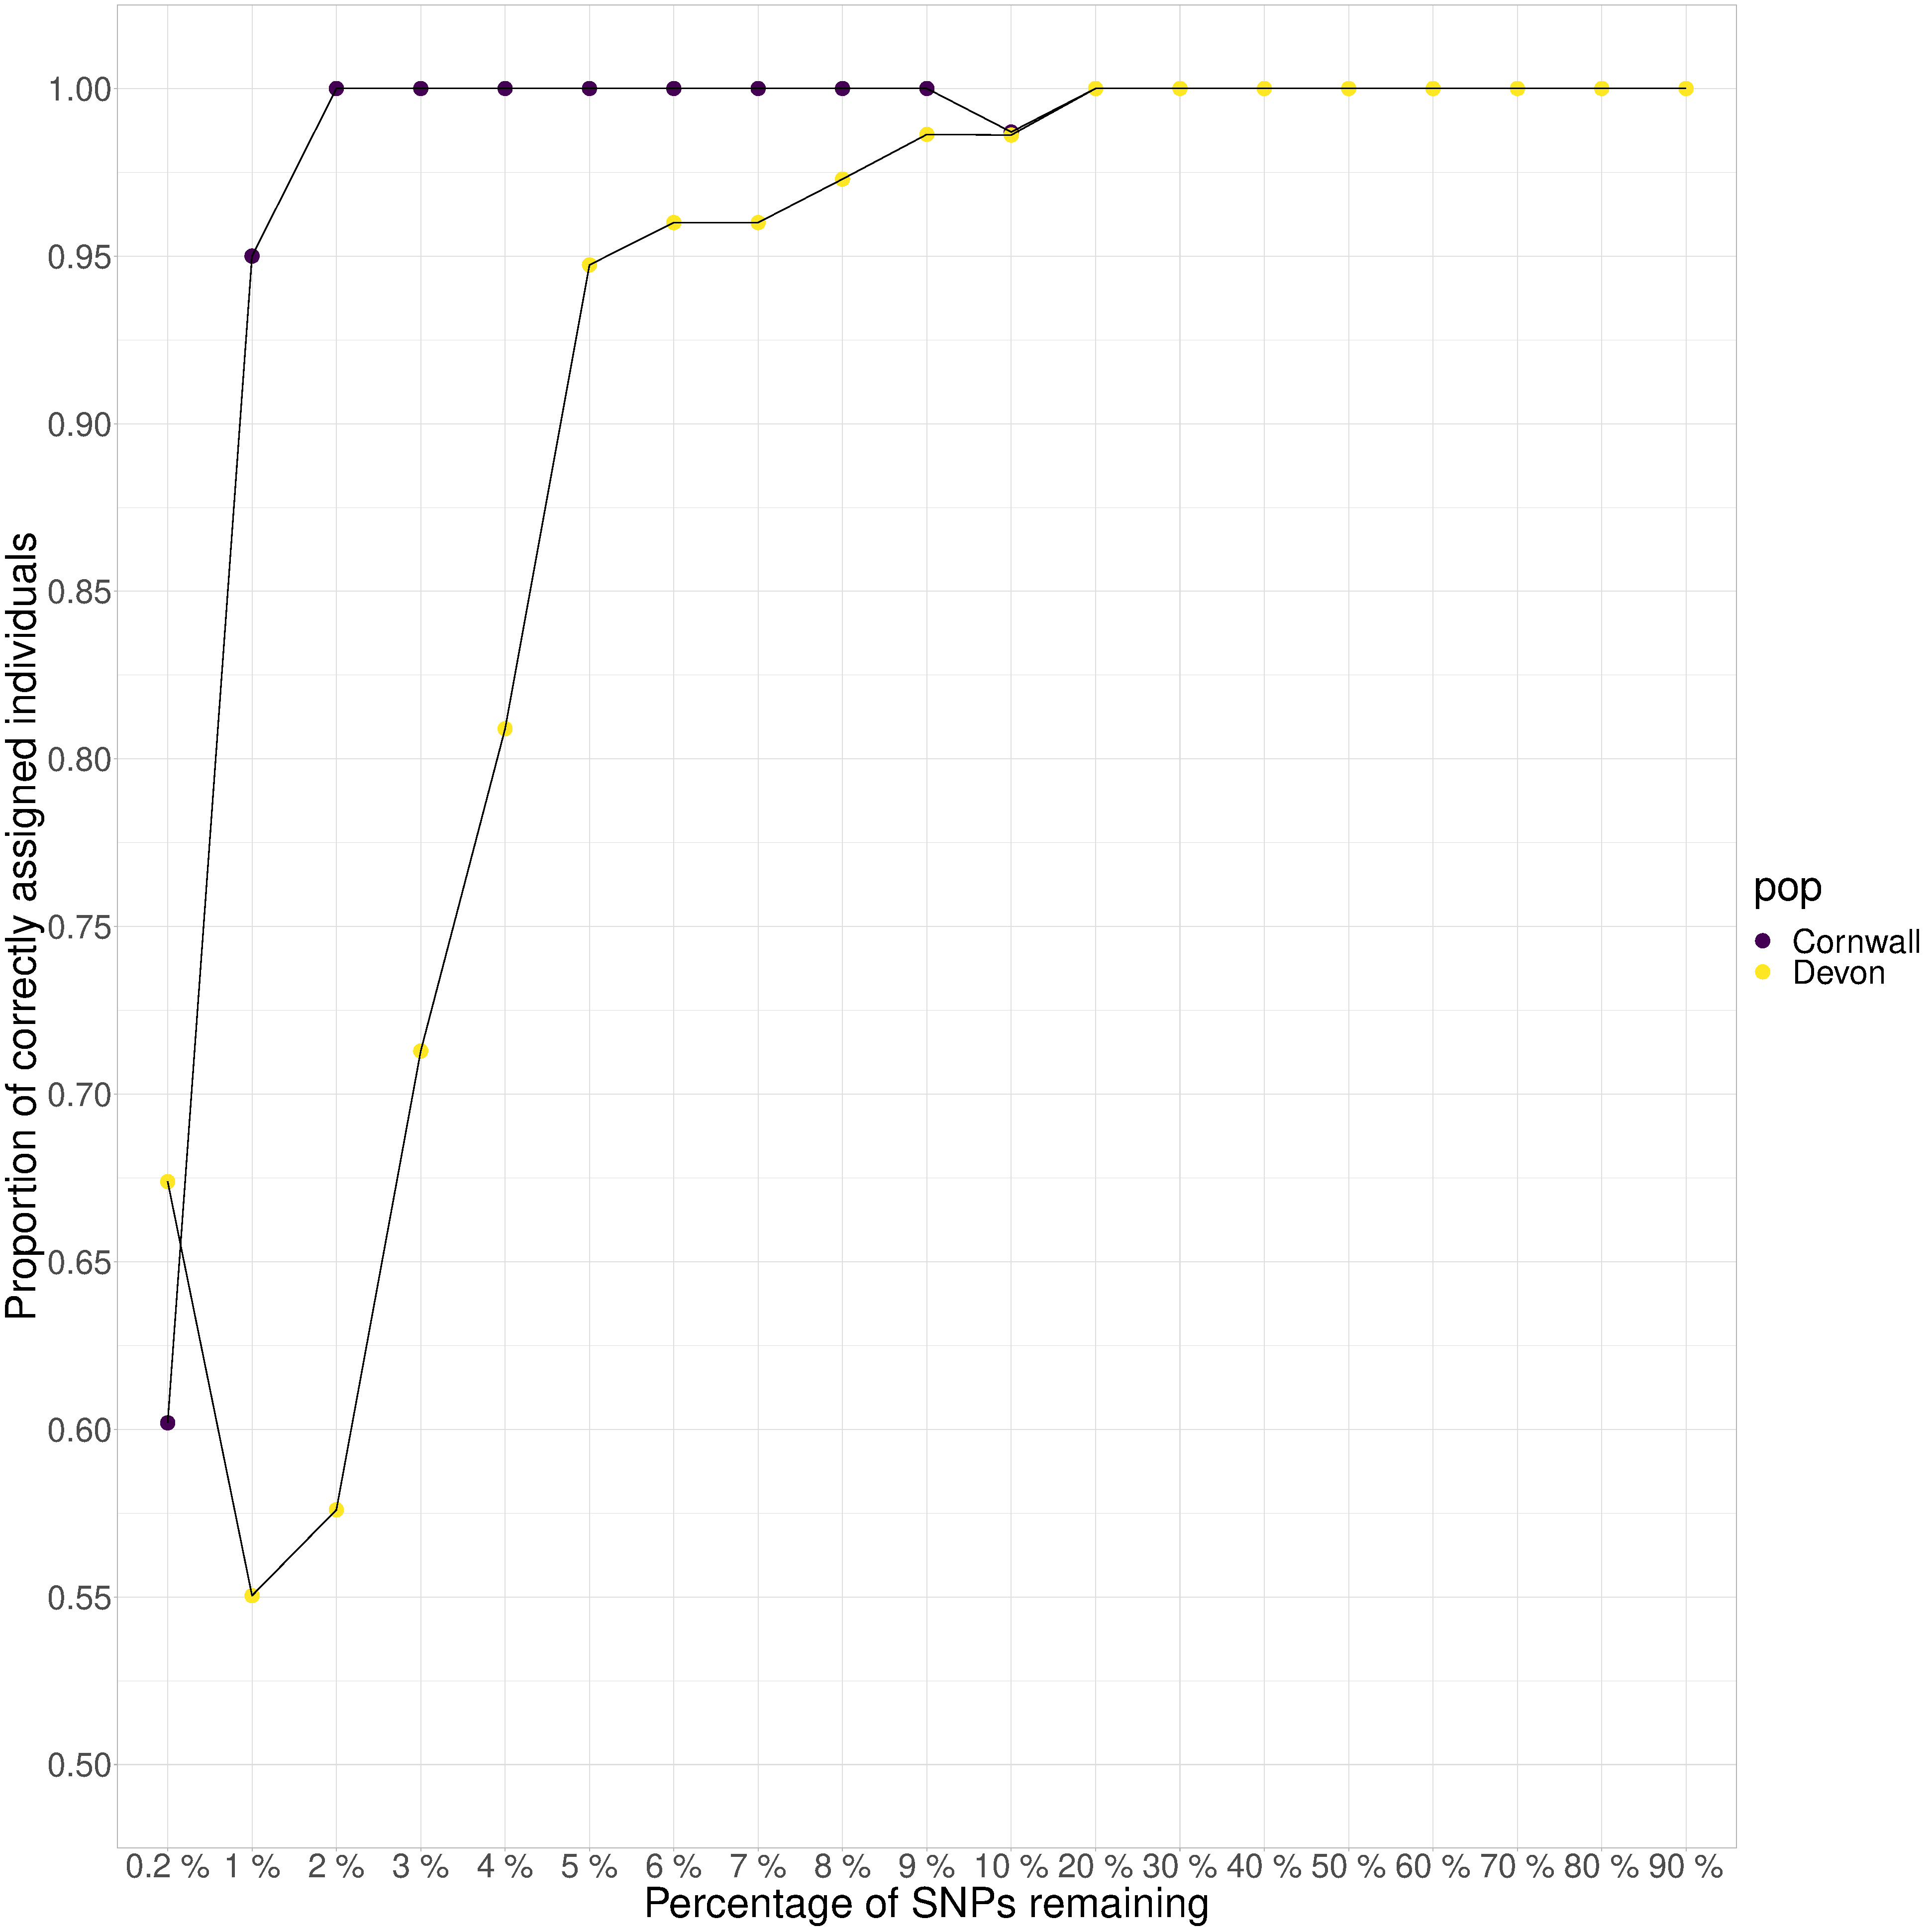
\includegraphics[width=1.0\textwidth]{../images/appendix/Devon_Cornwall_TVD_reduced.pdf}
    \caption{Proportion of individuals correctly assigned (via TVD) to their correct population (y-axis) using different number of SNPs (x-axis).}
    \label{fig:Devon_Cornwall_TVD_reduced_assignment}
\end{figure}
